\documentclass[unicode,master,printedition]{seuthesis} % 本科
% \documentclass[master]{seuthesis} % 硕士
% \documentclass[doctor]{seuthesis} % 博士
% \documentclass[engineering]{seuthesis} % 工程硕士
\usepackage{booktabs}
\usepackage{amsmath}
\usepackage{subfig}
\renewcommand\figureautorefname{图}
\renewcommand\tableautorefname{表}
%\usepackage{graphicx}
\DeclareGraphicsExtensions{.jpg,.pdf}
\graphicspath{{fig/}{figure/}{images/}}
%\hypersetup{unicode=false}
\setcounter{totalnumber}{8}
 % 这里是导言区

\begin{document}
\categorynumber{U121} % 分类采用《中国图书资料分类法》
\UDC{625}            %《国际十进分类法UDC》的类号
\secretlevel{公开}    %学位论文密级分为"公开"、"内部"、"秘密"和"机密"四种
\studentid{082200}   %学号要完整,前面的零不能省略。
\title{驾驶人行为特性对交通流的影响研究}{}{Study on the Impact of Driver Behavior Characteristics on Traffic Flow}{}
\author{吴\quad{}璠}{WU Fan}
\advisor{陆\quad{}建}{教授}{LU Jian}{Prof.}
%\coadvisor{副导师}{副教授}{Co-advisor's Name}{Associate Prof.} % 没有
                                % 可以不填
% \degree{工学硕士} % 详细学位名称
\major[12em]{交通运输规划与管理}
\defenddate{}
\authorizedate{}
%\department{交通学院}{Trasnportation College}
%\duration{2007.11—2008.6}
%\address{河海院2楼}
\maketitle

\begin{abstract}{驾驶人行为,交通流,驾驶人差异性,期望速度,减速度}
驾驶人是道路交通系统中最活跃的要素。不同驾驶人驾驶行为存在差异,同一名驾驶人在不同的外部环境和自身状态下的驾驶行为也不同。长期以来,我国机动车驾驶人均为专业驾驶人,随着大量小汽车进入家庭,产生了大量的非专业驾驶人。非专业驾驶人驾驶操作行为方面与专业驾驶人都存在差异。通过研究驾驶人行为特性及其对交通流的影响,将有助于对驾驶特性、驾驶行为与道路交通流的影响关系有更加深刻的理解。

本文分别以专业和非专业驾驶人为研究对象,选择典型的城市道路,在良好天气条件下,通过使用GPS和激光测距仪的跟车实验采集实际交通流状态下驾驶人的跟车速度、跟车间距、加速度等驾驶行为的主要参数。根据实验所得的测试车轨迹数据与其邻近车辆的相对速度和相对位置的时间序列数据,分析了驾驶人在真实驾驶环境中的自由行驶与跟驰的临界点特性、跟驰距离选择、加速度选择特性。通过对数据的集计分析以及跟驰模型的参数标定,分析并比较了驾驶过程中的不同驾驶人行为的异同。最后应用交通仿真程序SUMO,针对不同情况分别进行模拟研究。通过对驾驶人模型参数以及不同类型驾驶人混合比例的调整,研究了驾驶人行为特性对路段交通流的效率和安全特性的影响。

研究结果表明专业和非专业两组驾驶人的跟驰与自由流临界点特性方面存在差异。参数标定结果表明,驾驶人在期望速度和最大减速度方面存在差异。模拟研究发现,期望车速的改变对速度流量基本图上的曲线形状产生影响,且这种影响主要在自由流阶段。期望速度的增加导致碰撞时间TTC倒数的绝对值的时间平均值增加,这表明期望速度的增加对交通流的安全性存在负面影响。最大减速度的增加导致密度流量图上较难达到通行能力的区域。随着最大减速度的增加TTC倒数绝对值呈现先减小后增大的趋势,这表明存在不同最大减速驾驶人的最佳混合比例,从而使得TTC倒数绝对值的时间密度最小。专业驾驶人(低期望速度,高最大减速度)的增加导致相同流量下TTC倒数绝对值的最大值增加,交通流偏向不安全的方向。

本文的结果表明期望车速及最大减速度对交通流的效率性及安全性存在不同特点和程度的影响,而主要的影响因素是驾驶人的最大减速度。现有证据表明驾驶人行为特性对交通流的效率性和安全性存在不可忽略的影响。
\end{abstract}

\begin{englishabstract}{driver behavior, traffic flow, driver heterogeneity, desired speed, deceleration rate}

Driver is the most active part of road traffic system. Different drivers differ in driving behaviors, a driver also adapts his behavior to different external or internal states. For a long time in China, all drivers are professional drivers. However, with the boom of private cars, a lot of regular drivers emerged. Regular drivers show different driving behaviors in comparison with professional drivers. It is hopefully that through the investigation of the impact of driver behavior characteristics on traffic flow, a better understanding of driver behavior characteristics and the connection between driver behavior and traffic flow will be achieved.



Based on the assumption that driving experiences will alter drivers' behavior. A field car-following experiment featuring GPS and laser ranging was carried out to collect information about driver behaviors for both professional and regular drivers. 26 drivers recruited in the experiment were monitored for their speed, acceleration and following distance while they drove the experiment car on typical urban road in good weather conditions. After acquiring the trajectory and related data, aggregate analyses on the separation point of free driving and car-following , speed versus following distance,acceleration versus relative motion and model calibration were performed to investigate the heterogeneity of drivers' behaviors across the professional and regular driver groups. Finally, traffic simulation based on the SUMO software package was performed to asses the impact of 3 effects of driver behavior parameters' variations and combinations on traffic flow efficiency and safety measures.



Aggregate analyses suggest a difference in the separation point of free driving and car-following across the two driver groups. The results for model calibration suggest drivers have different desired speed and maximum deceleration rate. The simulation results indicate desired speed changes the shape of speed flow fundamental diagram in the free flow area. Higher desired speed increases the absolute value of time average inverse Time-to-Collision (abbreviated as |ITTC|/t), which means less safe. The increase of maximum deceleration rate (which is positive) makes it harder to reach the maximum capacity on density flow fundamental diagram. When the proportion of professional driver (with lower desired speed and higher maximum deceleration rate) increases, under same flow rate the maximum value of |ITTC| also increases, leading to a less safe state. However, there seem to be an optimal mixing rate of driver with different maximum deceleration rate where the |ITTC|/t is minimal.



In conclusion, both desired speed and maximum deceleration rate has impact on traffic flow efficiency and safety measures. And the main factor is maximum deceleration rate as its effects dominate the combined effects. Current evidences suggest there is a non-negligible effect of driver behavior characteristics on traffic flow.
\end{englishabstract}

%\begin{terminology}
%  本论文专用术语的注释表
%\end{terminology}

\begin{Main} % 开始正文

%\chapter{绪论(前言)}
%\section{研究的主要内容}
%\subsection{...}
%\subsubsection{...}
%\section{需要解决的问题}
%使得论文符合要求\cite{seugs:standard}。
%
%\chapter{...}
%...
\chapter{绪论}
\section{主要研究内容}
这是测试\cite{seugs:standard}
\chapter{驾驶人行为特性的内涵}



%\begin{table}[htbp]
% \centering
% \caption{Add caption}
% \begin{tabular}{cccc}
%   \addlinespace
%    \toprule
%    Face database & Yale  & Caltech & ORL \\
%    \midrule
%    Number of training & \multicolumn{ 1}{c}{5} & \multicolumn{ 1}{c}{3} & \multicolumn{ 1}{c}{3} \\
%    samples per class  & \multicolumn{ 1}{c}{} & \multicolumn{ 1}{c}{} & \multicolumn{ 1}{c}{} \\
%    \bottomrule
%    \end{tabular}
%  \label{tab:addlabel}
%\end{table}

\section{跟驰行为特性}
\subsection{跟驰行为特性参数}
\subsection{跟驰行为差异性}
\subsubsection{跟驰行为内部的差异性}
\subsubsection{驾驶人之间跟驰行为的差异性}
\subsubsection{不同跟车对的跟驰行为的差异性}

\section{变道行为特性}


\chapter{驾驶人行为特性实验}


%\[D = ct/2\]




\section{有关驾驶人行为特性实验方法回顾}

%\begin{equation}
%D = 2R{\rm{asin}}(\sqrt {\sin _{}^2(\frac{{{l_1} - {l_2}}}{2}) + \cos ({l_1})\cos ({l_2}){{\sin }^2}(\frac{{{w_1} - {w_2}}}{2})} )
%\end{equation}

\section{实验设计}
\subsection{实验目的}

调查专业驾驶人与非专业驾驶人在城市路段行车时,采取的驾驶行为的异同,为进一步分析驾驶人行为特性对城市路段交通流的影响提供数据。

\subsection{实验获取的数据}
分别获取单向两车道与三车道上,驾驶人行车过程中,本车与前后车实时保持的距离,即$S_{\text{前}}$、$S_{\text{后}}$;本车的实时速度$V$,前车的实时速度$V_{\text{前}}$;后车的实时速度$V_{\text{后}}$;本车与前车相对速度${\Delta}S_{\text{前}}$;本车与后车相对速度v’后;本车换道频率n,换道时相邻车道提供的前后车距离s换等。


\subsection{实验设备}
实验设备包括小汽车一辆(现代sonata手动档)、车载激光测速测距仪一体化系统一套(车载激光两台、GPS一个、处理机一台)、摄像机一台、笔记本电脑一台。
\begin{table}[htbp]
 \centering
 \caption{试验设备列表}
 \begin{tabular}{cccc}
   \addlinespace
    \toprule
    序号 & 名称  & 构成 & 用途 \\
    \midrule
	1 & 小汽车 & 北京现代sonata手动档 & 实验用车 \\
	2 & 车载激光测速测距仪 & 车载激光(两台)、GPS、处理机 & 获取实时车间距、相对速度 \\
	3 & 摄像机 & 摄像机 & 车辆换道行为监控 \\
	4 & 笔记本电脑 & Thinkpad T40笔记本 & 现场数据采集终端 \\
    \bottomrule
    \end{tabular}
  \label{tab:addlabel}
\end{table}

其中,小汽车选取目前道路上较为常见,比较有代表性的车型,北京现代的sonata领翔 2.0 GL MT,具体参数如表3-2.

\subsection{实验原理}
通过获取实时连续的本车与前后车的距离以及本车的实时速度,可以推算得到本车与前车和后车的相对速度、前后车的实时速度等相关数据,应用摄像机可以得到本车的换道频率,最后经过数据的处理分析,可以得到换道时本车道前后车的距离,以及换道时相邻车道提供的前后车距离等。
\subsubsection{激光测距基本原理}
激光测距仪是指利用射向目标的激光脉冲或连续波激光束测量目标距离的距离测量仪。它由三大部分组成:激光发射机、激光接收机、电源。激光发射机由脉冲激光器、发射光学系统、取样器以及瞄准光学系统组成,其作用是将高峰值功率的激光脉冲射向目标。激光接收机由接受光学系统、光电探测器和放大器、接收电路和计数显示器组成,其作用是接收从目标漫反射回来的激光脉冲回波并计算和显示目标距离。电源用于设备的供电。
激光测距仪的工作原理是利用脉冲激光器向目标发射单次激光脉冲,计数器测量激光脉冲到达目标并由目标 返回到接收机的往返时间,由此运算目标的距离。计算公式为:

\begin{equation}
D = ct/2
\end{equation}

其中$D$是与目标的距离, $c$为光速,$t$是光往返时间。

激光测距仪的工作过程是:首先瞄准目标,然后接通激光电源,起动激光器,通过发射光学系统,向瞄准的目标发射激光脉冲信号。同时,采样器采集发射信号,作为计数器开门的脉冲信号,起动计数器,钟频振荡器向计数器有效的输入钟频脉冲,由目标反射回来的激光回波经过大气传输,进入接收光学系统,作用在光电探测器上,转变为电脉冲信号,经过放大器放大,进入计数器,作为计算器的关门信号,计数器停止技术。计数器从开门到关门期间,所进入的钟频脉冲个数,经过运算得到目标距离,在显示器上显示出来。


\subsubsection{GPS卫星定位系统基本原理}
GPS系统由空间部分、地面监控部分和用户端三个部分组成。
(1)GPS的空间部分:由21颗工作卫星和3颗备用卫星组成,24颗卫星均匀覆盖在地球上空,可以保证地球上所有地点任意时刻都能同时看到至少4颗GPS卫星。
(2)GPS的地面监控部分:地面监控设备的作用是监测和控制卫星上的各种设备是否正常工作,以及卫星是否一直沿着预定轨道运行;另一作用是保持各颗卫星处于同一时间标准——GPS时间系统。GPS地面监控系统包括一个主控站、三个注入站和五个监测站。
(3)GPS的用户端:即是GPS的信号接收机,它能捕获卫星的信号,对所接收的GPS信号进行变换、放大和处理,实时地计算出测点的三维位置、速度和时间。
GPS系统的基本原理是:太空中的卫星在任意时刻都有一个坐标值(已知值),接收机所在位置为未知值,信息在传送过程中,所需耗费的时间,可经由比对卫星时钟与接收机内的时钟计算之,将此时间差值乘以电波传送速度(一般为光速),就可计算出卫星与接收机间的距离,如此就可依三角向量关系来列出一个相关的方程式,每接收到一颗卫星就可列出一个相关的方程式,因此收到至少三颗卫星信号,即可计算出经纬度坐标,收到四颗则加上高程值,五颗以上更可提高准确度。当接收机处于动态时,每一秒钟的坐标数据都在更新中,也就是说接收机会自动不断地接收卫星信号,并实时地计算其所在位置的坐标数据。系统再将获取的空间与时间的数据结合,计算出车辆的实时速度。

\subsubsection{车载GPS定位仪系统工作流程}
驾驶人在道路上行驶时,车载GPS实时接收卫星信号,经过计算获取车辆实时的精度与纬度,然后将数据传导至处理机,经过处理机运算处理后,计算出车辆的实时速度,最后将实时坐标数据与实时车辆速度传到与处理机相连的笔记本电脑中,为后续的数据处理提供原始资料。车载GPS卫星定位仪工作流程如图3-1所示。

\subsubsection{车载激光测距系统}
激光间距测量仪相比其它测距仪,激光测距仪具有测距精度高、测距速度快、轻小灵活、测量距离数字显示、操作简单等优点。下面分别介绍车载激光的硬件系统和软件系统。
(1)硬件系统
车载激光硬件系统包括激光接收发射一体化系统、车载电源线、输出终端(笔记本)及相关配套设施。其中激光发射机、接收机是车载激光系统的主体设备,封装于一台设备中。给设备连接于一台处理机上,处理机经过计算,将获取的数据发送到笔记本电脑上显示,处理机另外外接两条线,一条是车载电源线,与12V的车载电源连接;另一条是数据线缆,与笔记本相连,与笔记本相连的一端采用了USB2.0 to SR232转换接口。硬件系统模式见图3-2。
(2)软件系统
由激光测距工作过程知,脉冲个数的读取及目标距离需要通过运算得到。北京奥泽尔科技有限公司为本次试验专门开发了一个为计算车头间距的激光测距软件。

\subsubsection{仪器安装}
仪器的安装如图3-4所示。一个车载激光固定在实验车辆挡风玻璃后面,中控台中央的位置,激光头向前放置,能够使激光照射到实验车辆前方的物体;另一个车载激光固定在后车窗玻璃以内,激光头向后放置,透过后车窗玻璃使激光能够照射到实验车辆后方的物体;车载GPS固定在车辆中将的位置;处理机和笔记本电脑放置在车辆后排座位上;摄像机固定在实验车辆后排座位靠背的中间位置上,可以通过实验车辆挡风玻璃拍摄到前方的道路交通情况。

\subsubsection{数据处理}
通过实验仪器获取的数据只有实验车辆与前车和后车的实时距离,以及实验车辆的实时经纬度,要得到我们所需要的实验车辆速度、前车相对速度、前车速度、后车相对速度、后车速度等数据,可以通过以下计算得到。
GPS定位仪输出的是WGS-1984经纬度坐标,在此坐标下计算行驶距离的公式为:
\begin{equation}
D = 2R{\rm{asin}}(\sqrt {\sin _{}^2(\frac{{{l_1} - {l_2}}}{2}) + \cos ({l_1})\cos ({l_2}){{\sin }^2}(\frac{{{w_1} - {w_2}}}{2})} )
\end{equation}
其中 $D$(m)为经纬度坐标点( ${l_1},{w_1}$)和(${l_2},{w_2}$)之间的距离, $R$为地球半径,取6378137m。设定GPS每秒钟返回一个数据,当前车辆的瞬时速度 (单位m/s)计算公式为:$v = D'$
设$\Delta t$为记录前后两个坐标点的时间差,本车加速度 $a$($m/s^2$)则通过本车速度计算得到,计算公式为:
\begin{equation}
a = \frac{{{v_1} - {v_2}}}{{\Delta t'}}
\end{equation}
其中$v_1$,$v_2$分别为相邻的两瞬时速度(单位m/s), $\Delta {t'}$为两个瞬时速度的时间差(单位s)。激光测距仪直接输出的是本车车头与前车车尾之间的间距,前车与本车的相对速度 (m/s)计算公式如下:
\begin{equation}
{v_r} = \frac{{{d_2} - {d_1}}}{{\Delta {t^{''}}}}
\end{equation}
其中$d_1$,$d_2$为相邻两个车间距(单位m), $\Delta t''$为两个相邻车间距对应的时间差(单位s),又${v_r} = {v_f} - {v_b}$,其中${v_f}$为前车速度(单位s), ${v_b}$为后车速度(单位s),故前车的速度为:
\begin{equation}
{v_f} = {v_r} + {v_b}
\end{equation}

\subsection{实验方法}
\subsubsection{实验对象}
实验对象分为专业驾驶人与非专业驾驶人,各十五人。其中,专业驾驶人主要选取长期从事驾驶工作,或驾龄7年且累计行程10万公里以上的驾驶人;非专业驾驶人主要选取非特定职业,驾龄不足7年或累计行程不足10万公里的驾驶人。选取的专业驾驶人与非专业驾驶人都尽可能来自各行各业,覆盖各年龄层,男女比例均衡。
\subsubsection{实验路线}
实验路线的选取要注意多项条件。首先,道路条件方面应包含单向两车道城市道路与单向三车道城市道路,且路段上开口较少,有机非分隔带,机动车行驶受非机动车和行人干扰较小,路面情况良好;其次,交通条件方面要有足够大的交通流量,但是不至于造成长时间的拥堵,道路上行驶的车型以小汽车为主。
经过实地调查分析,本实验选取的实验路段为:南京市龙蟠中路-瑞金路-御道街-中山东路一线。其中龙蟠中路为双向六车道;瑞金路东西向为三车道,西东向为两车道;御道街靠近瑞金路一段为双向四车道,靠近中山东路一段为双向六车道;中山东路为双向四车道。该路段全天交通流量均较大且高平峰时流量相差不大,平峰时段车流量满足要求,高峰时段不造成长时间拥堵,车辆跟驰特征明显,比较符合实验要求。具体线路如图3-5所示。

\subsubsection{实验条件}
天气状况良好、无大风大雨、光线充足的情况下,分别在工作日与非工作日的交通流量较大的时候进行实验。所选取的时间段主要在车流量较大但不造成长时间拥堵的时候,能够满足车辆跟驰的要求。经过调查发现,在该路段上,工作日与非工作日的交通流量变化不大,交通流量与高平峰时间段相对固定。最后根据所选取路段的交通流量以及高平峰的时间,本论文实验时间定为8:00——11:00和13:00——18:00。
\subsubsection{实验过程}
首先,每个实验参与者在按照既定路线驾驶行车前,先进行简单培训,说明本次实验的目的、设备的安置及用途、既定的路线等,使实验参与者对本实验有个理性的认识,有助于本次实验的顺利开展。
其次,将我们准备好的《驾驶人特性实验调查问卷》与《驾驶人安全意识调查表》给实验参与者填涂。
具体表格(暂略待补)
然后,开始进行路上实验,由一名实验参与者按照事先拟定的路线,驾驶实验车辆,沿着龙蟠中路——瑞金路——御道街——中山东路——龙蟠中路一圈后调头,再沿着龙蟠中路——中山东路——御道街——瑞金路——龙蟠中路行驶。
最后,保存数据,结束一次实验。
准备下一个实验参与者进行实验。





















%\begin{table}[htbp]
% \centering
% \caption{Add caption}
% \begin{tabular}{cccc}
%   \addlinespace
%    \toprule
%    Face database & Yale  & Caltech & ORL \\
%    \midrule
%    Number of training & \multicolumn{ 1}{c}{5} & \multicolumn{ 1}{c}{3} & \multicolumn{ 1}{c}{3} \\
%    samples per class  & \multicolumn{ 1}{c}{} & \multicolumn{ 1}{c}{} & \multicolumn{ 1}{c}{} \\
%    \bottomrule
%    \end{tabular}
%  \label{tab:addlabel}
%\end{table}

\chapter{驾驶人行为特性的差异性分析}
\section{数据处理}
\subsection{数据构成}
\subsection{数据筛选}

\section{跟驰行为特性的差异}


\subsection{时间间隔分布}
时间间隔的定义:
取20s以内的时间间隔数据,非专业驾驶人时间间隔分布如图4.1,专业驾驶人时间间隔分布如图4.2。使用对数正态分布进行拟合,0.05显著水平下,卡方检验均不符合对树正态分布,KS检验专业驾驶人符合对数正态分布,非专业驾驶人不符合对数正态分布。专业驾驶人时间间隔整体上小于非专业驾驶人的时间间隔,这符合一般的感性认识。


\subsubsection{非专业}
\begin{figure}[htpb]
	\centering
	\label{tgap_distru:non_pro}
	\includegraphics[totalheight=10cm]{o1}
	\caption{非专业驾驶人时间间隔分布}
\end{figure}


Distribution:    Lognormal\\
Log likelihood:  -11056.3\\
Domain:          0 < y < Inf\\
Mean:            4.37392\\
Variance:        18.3609\\

Parameter  Estimate  Std. Err. \\
mu          1.13926   0.0119837\\
sigma      0.820249  0.00847512\\

Estimated covariance of parameter estimates:\\
       mu            sigma       \\
mu      0.000143609  1.51271e-019\\
sigma  1.51271e-019  7.18276e-005\\

检验\\
Chi-square:\\
null hypothesis :服从lognormal分布\\
p= 1.74778427653571e-27<0.05 拒绝\\
KS-test:\\
null hypothesis :服从lognormal分布\\
p= 1.24971275593801e-13<0.05 拒绝\\






\subsubsection{专业}
\begin{figure}[htpb]
	\centering
	\label{tgap_distru:pro}
	\includegraphics[totalheight=10cm]{o2}
	\caption{专业驾驶人时间间隔分布}
\end{figure}

Distribution:    Lognormal\\
Log likelihood:  -8615.43\\
Domain:          0 < y < Inf\\
Mean:            4.43296\\
Variance:        22.3341\\

Parameter  Estimate  Std. Err.\\
mu          1.10947  0.0145138\\
sigma      0.871312  0.0102649\\

Estimated covariance of parameter estimates:\\
       mu             sigma        \\
mu        0.00021065  -2.79065e-019\\
sigma  -2.79065e-019    0.000105369\\


检验\\
Chi-square:\\
null hypothesis :服从lognormal分布\\
p= 2.17243543058168e-13<0.05 拒绝\\

KS-test:\\
null hypothesis :服从lognormal分布\\
p= 0.0575478261225268>0.05 接受\\

\subsection{速度--跟驰距离}
对于每一个驾驶人根据速度划分区间对跟车速度和跟驰距离进行平均,得到平均意义上的跟车速度和跟驰距离,从图4.3和图4.4可以看出,无论是非专业还是专业驾驶人,在图形下方均有一条较为明显的趋势线呈现相对线性的关系,同时均存在较大的变化,表明跟驰行为中存在驾驶人其跟车速度和跟驰距离较为偏离线性关系这一假设。从图中看专业驾驶人的变化情况似乎大于专业驾驶人,可以推测专业驾驶人存在更多的不同驾驶类型。
\begin{figure}[htpb]
	\centering
	\label{spd_dist:nonpro}
	\includegraphics[totalheight=10cm]{non_spd_dist}
	\caption{非专业驾驶人速度--跟驰距离}
\end{figure}



\begin{figure}[htpb]
	\centering
	\label{spd_dist:pro}
	\includegraphics[totalheight=10cm]{pro_spd_dist}
	\caption{专业驾驶人速度--跟驰距离}
\end{figure}

\begin{figure}[htpb]
	\centering
	\label{spd_dist:all}
	\includegraphics[totalheight=10cm]{all_spd_dist}
	\caption{专业、非专业驾驶人速度--跟驰距离比较}
\end{figure}



\subsection{加速度--相对速度}

对于每一个驾驶人根据相对速度划分区间对加速度和相对速度进行平均,得到平均意义上的加速度和相对速度,从图4.6和图4.7可以看出,无论是非专业还是专业驾驶人,从整体趋势上呈现左低右高,意味着本车速度大于前车速度时有减速的趋势,反之亦反。而图中没有呈现明显的线性变化,而是呈现较大的随机性,跟驰模型中一般假设驾驶人加速度与速度差紧密相关,虽然其具有良好的数学特性,但是实际情况中驾驶人具有非即时反应性,有计划性,这一假设相比于速度与跟驰距离的假设而言是较为严格的假设。同时从图中可以看出代表不同驾驶人的折线变化较大,这表明驾驶人的驾驶类型存在较大差异。
\begin{figure}[htpb]
	\centering
	\label{rspd_acc:nonpro}
	\includegraphics[totalheight=10cm]{non_rspd_acc}
	\caption{非专业驾驶人加速度--相对速度}
\end{figure}

\begin{figure}[htpb]
	\centering
	\label{rspd_acc:pro}
	\includegraphics[totalheight=10cm]{pro_rspd_acc}
	\caption{专业驾驶人加速度--相对速度}
\end{figure}

\begin{figure}[htpb]
	\centering
	\label{rspd_acc:all}
	\includegraphics[totalheight=10cm]{all_rspd_acc}
	\caption{专业、非专业驾驶人加速度--相对速度比较}
\end{figure}

%\subsection{速度、加速度特性差异}
%
%\subsection{跟驰距离特性差异}
%\subsection{时间间隔特性差异}
%\begin{figure}[htpb]
%\includegraphics[totalheight=10cm]{Graph1}
%\end{figure}
\subsection{对不同跟驰模型的参数标定及其表现比较}
不同的跟驰模型的不同假设,可以体现驾驶人的不同驾驶类型。通过每条跟驰轨迹使用不同跟驰模型的参数标定,并进行模型拟合程度表现的比较,可以定量化的研究驾驶人的驾驶类型差异。

本文中将选取
\subsubsection{各模型简述}
\subsubsection{轨迹数据的平滑处理}
\subsubsection{参数标定方法}
\subsubsection{模型拟合程度的量化}
\subsubsection{比较结果}




\section{变道选择与间隙接受特性差异}

\section{驾驶人行为特性相关性分析}
\chapter{驾驶人行为特性对交通流影响}
\section{研究框架}
为了研究驾驶人行为特性对交通流的影响,由于交通流的复杂性。同时由于道路上的驾驶人个体,很难对其进行逐个的观测与调查,本文使用微观模拟的方法对驾驶人行为特性对交通流影响进行研究。
\subsection{模拟软件sumo简介}

根据Krajzewicz等(2006)\cite{Krajzewicz2006}
2000年起,德国航空中心(DLR)的交通研究所(IVF)开始开发微观交通模拟软件。并以开源的形式发布了整个软件包SUMO,作为交通研究中算法和模型的一般测试平台。SUMO为“Simulation of Urban MObility”的缩写,SUMO已被应用于模拟Magdeburg和Cologne,其研究主要关于交通管理和交通预测。

根据Krajzewicz等(2005)\cite{Krajzewicz2005},SUMO的默认值使用了Krauß跟驰模型,Krauß(1998)\cite{Krauss1998}提出了一个微观的空间连续跟驰模型,其主要基于安全速度假设,驾驶人为了对前车减速保有一定的安全余量,选择一定的距离和安全速度。模型假设驾驶人的反应时间tau为1s。并且SUMO可以很好的重现密度流量关系图。

\begin{figure}[!htb]
\begin{center}
\includegraphics[width=\linewidth]{sumo}
\end{center}
\caption{sumo模拟密度-流量例图(摘自Krajzewicz等(2005)\cite{Krajzewicz2005})}
\label{sumo}
\end{figure}

Krauß模型给出如下:

\begin{equation}
v_{safe}=v_l(t)+\frac{g(t)-v_l(t)\tau}{\frac{\bar{v}}{b(\bar{v})}+\tau}
\end{equation}

其中:
\begin{displaymath}
{\begin{aligned}
v_l(t)&-t\text{时刻前车速度}\\
g(t)&-t\text{时刻与前车的空间间隔}\\
\tau&-\text{驾驶人的反应时间}\\
b&-t\text{减速函数}\\
\end{aligned}}
\end{displaymath}

为了保证车辆不超过其物理加速能力和最大速度,计算$v_{des}(t)$
\begin{equation}
v_{des}(t)=min[v_{safe},v(t)+a,v_{max}]
\end{equation}

最后从期望速度中减去随机项,使得模型变为随机
\begin{equation}
v_{t}(t)=max[0,rand[v_{des}(t)-\epsilon a,v_{des}(t)]]
\end{equation}



有效性

Ossen(2008)\cite{Ossen2008}研究表明,通过Gipps模型构造的人造轨迹数据对Tampère进行参数标定,结果表明即使模型不同,只要有足够的观测,仍可以对驾驶人的跟驰行为得出相似的理解。由于不存在完美的跟驰模型,但是人可以从实际观测数据对驾驶人行为作相互合理推断,同时相似结构的模型均可以揭示出驾驶人的行为特征。
因此,从前一章根据IDM模型得出的驾驶人差异性的结论仍可以认为对其他模型是成立的。

% Based on these results it seems justified to conclude that the true car-following behavior of the 
% observed follower can be identified by calibrating an “imperfect” model. 



Kerner\cite{S.Kerner2009}认为,传统的基于基本图的交通流理论不能解释,高速公路交通流的实际观测到的拥堵现象,提出了三相交通流理论。Kerner认为由于传统跟驰模型不能重现实际观测中的散落的密度-流量基本图,这一观点被Helbing认为是错误的,其评论Krauß模型认为由于Krauß模型,不能构成其认为的不连续超车概率因此不能解释F-S和S-J的相位变化。

Schönhof和Helbing\cite{Schoenhof2009}指出传统跟驰模型不能重现实际观测中的散落的密度-流量基本图,是由于未考虑驾驶人驾驶行为的差异性,传统模型的混合驾驶人模拟被证明可以重现实际观测中的散落的密度-流量基本图。


% IDM implementation

\subsection{模拟场景}


如图中,本文模拟场景设置为600m直线路段,单向3车道,为了增加扰动在路段末端设为2车道.共设置6个线圈检测器,分别在150m处和450m处。

\begin{figure}[!htb]
\begin{center}
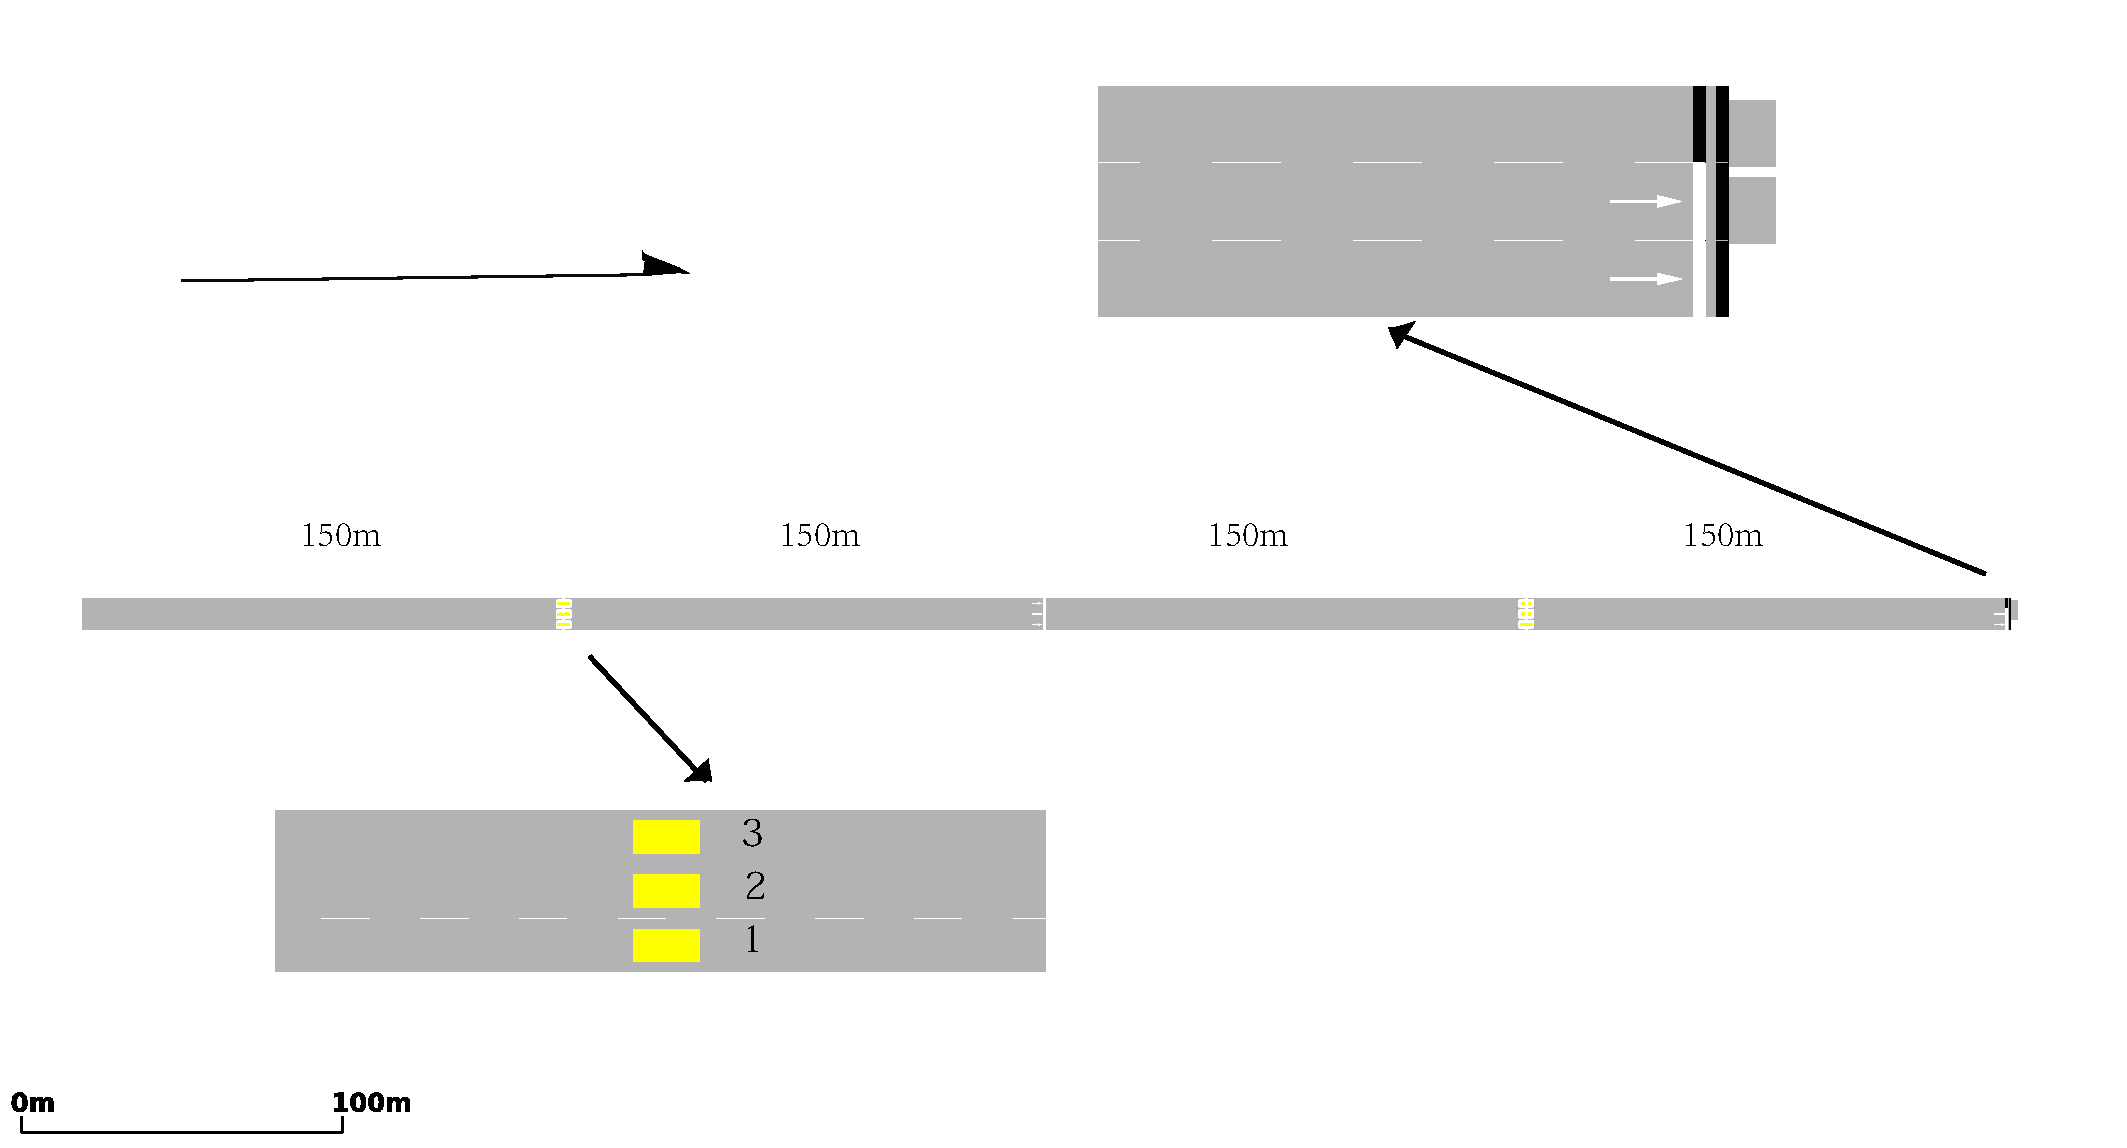
\includegraphics[width=\linewidth]{scene}
\end{center}
\caption{模拟场景图}
\label{scene}
\end{figure}

输入的交通流量,设置0-1200s,流率为600,1200-2400s,流率为1800,2400-4800s,流率为600,如\autoref{input-demand}

\begin{figure}[!htb]
\begin{center}
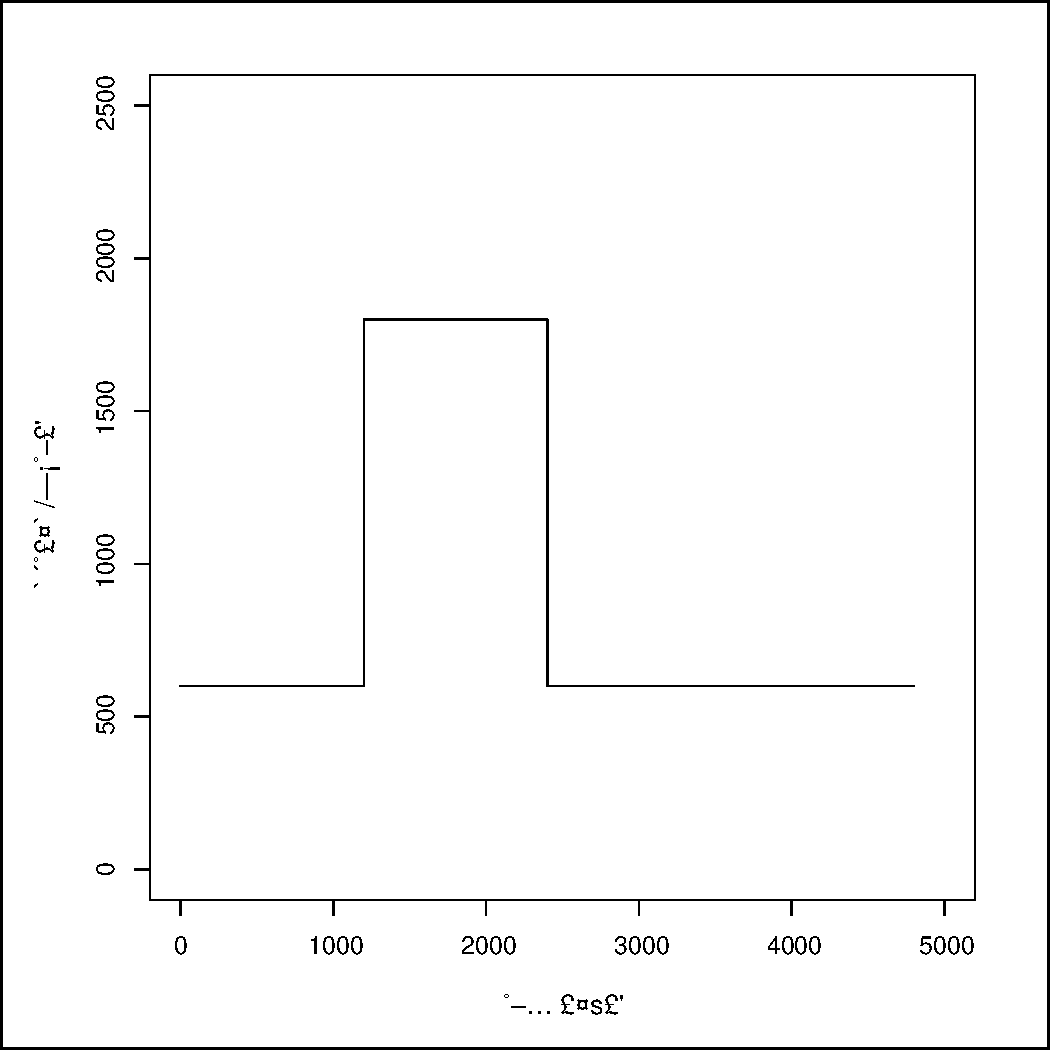
\includegraphics[width=0.3\linewidth]{input-demand}
\end{center}
\caption{交通需求随时间变化图}
\label{input-demand}
\end{figure}

为了研究驾驶人行为特性对交通流的影响,结合第四章所得结论。主要考察三种效应的影响,一为驾驶人期望车速对交通流的影响,二是驾驶人最大减速度对交通流的影响,三为两者混合效应的影响。

针对三种效应,对每一种效应分别选择两种车型,以全部A类型驾驶人,1:3,1:1和3:1的比例混合和全部B类型驾驶人分别进行模拟,也就是说B类型的驾驶人从0\%到25\%,50\%,75\%增加到100\%,由于在驾驶人混合中,车辆的出发顺序随机,在驾驶人混合中以不同随机种子数模拟10次。

\begin{table}[htb] 
  \begin{minipage}[b]{0.25\linewidth} 
  \centering
  \caption{期望速度的效应}
    \begin{tabular}{rrr}
    \addlinespace
    \toprule
    驾驶人类型    & A     & B \\
    \midrule
    最大加速度 & 0.62  & 0.62 \\
    最大减速度 & 2.33  & 2.33 \\
    期望速度  & 6.48  & 8.09 \\
    \bottomrule
    \end{tabular}%
  \label{speed-factor}%
  \end{minipage}% 
\hspace{0.08\linewidth}
  \begin{minipage}[b]{0.25\linewidth} 
  \centering
  \caption{最大减速度的效应}
    \begin{tabular}{rrr}
    \addlinespace
    \toprule
    驾驶人类型    & A     & B \\
    \midrule
    最大加速度 & 0.62  & 0.62 \\
    最大减速度 & 2.33  & 4.29 \\
    期望速度  & 8.09  & 8.09 \\
    \bottomrule
    \end{tabular}%
  \label{decel-factor}%
  \end{minipage}
\hspace{0.08\linewidth}
  \begin{minipage}[b]{0.25\linewidth} 
  \centering
  \caption{混合效应}
    \begin{tabular}{rrr}
    \addlinespace
    \toprule
    驾驶人类型    & A     & B \\
    \midrule
    最大加速度 & 0.62  & 0.62 \\
    最大减速度 & 2.33  & 4.29 \\
    期望速度  & 8.09  & 6.48 \\
    \bottomrule
    \end{tabular}%
  \label{combined-factor}%
  \end{minipage} 
\end{table}






\subsection{评价指标}
效率性,主要从基本图来看交通流效率性的影响
安全性,以TTC倒数的和来评价安全性


\section{对交通流效率性}

\subsection{期望速度影响因素}
根据\autoref{speed-factor}的驾驶人参数进行混合模拟,得到:

\begin{figure}[!htb]
\begin{center}
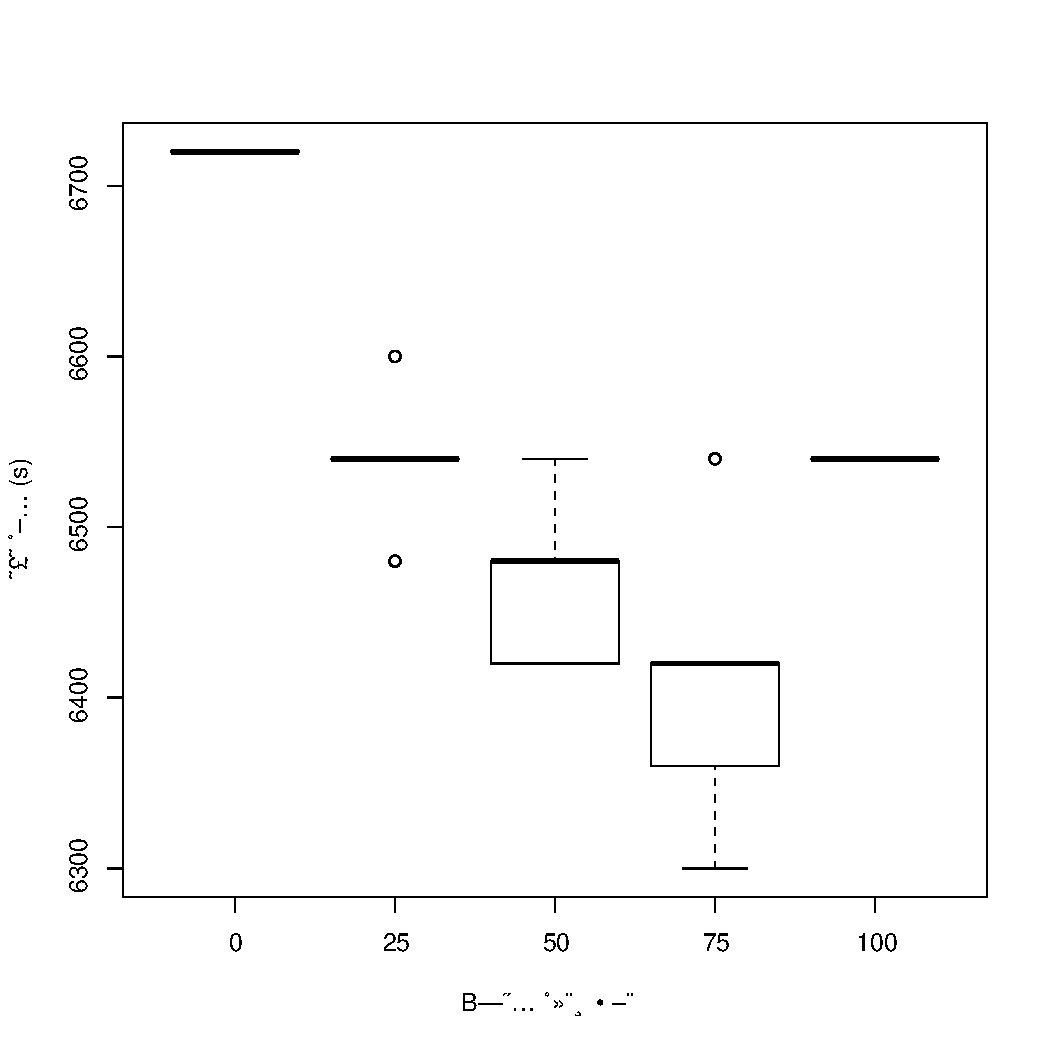
\includegraphics[width=0.5\linewidth]{factor1_box_ttime}
\caption{期望速度影响下模拟用时箱图}
\label{factor1_box_ttime}
\end{center}
\end{figure}

\autoref{factor1_box_ttime}给出了,期望速度影响下模拟总用时的变化,随着\autoref{speed-factor}中期望速度较大的B型驾驶人的增加,模拟所用时间呈现下降的趋势。对于单纯类型的驾驶人组合,期望速度由6.48m/s(23.3km/h)增加8.09m/s(30.6km/h),增加24.8\%,模拟用时从6720s下降到6540s,降低了3\%。

对速度-流量图形状的影响


\begin{figure}[!htb]%
\centering
\subfloat[][]{
\label{factor1_vq_per0}%
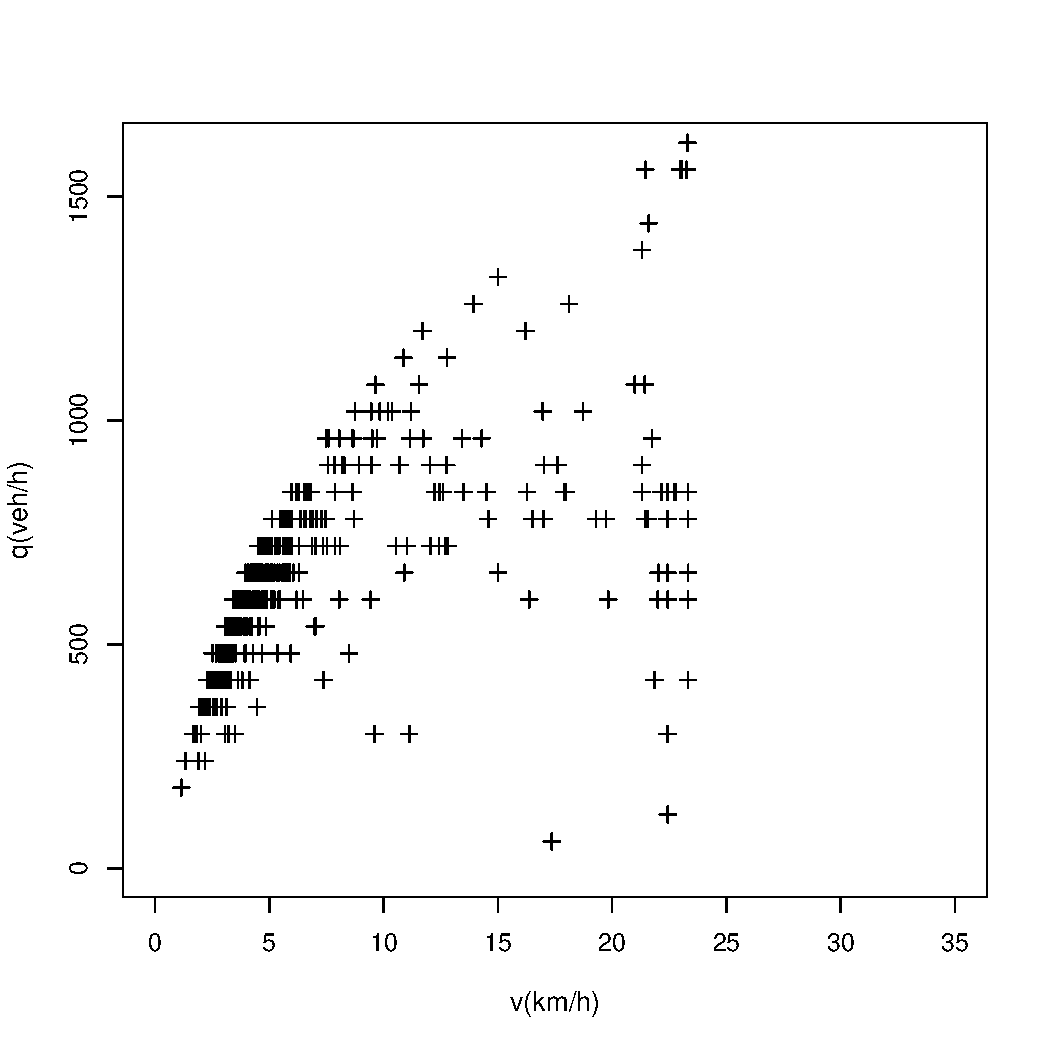
\includegraphics[width=0.33\linewidth]{factor1_vq_per0}
}%
\subfloat[][]{%
\label{factor1_vq_per25}%
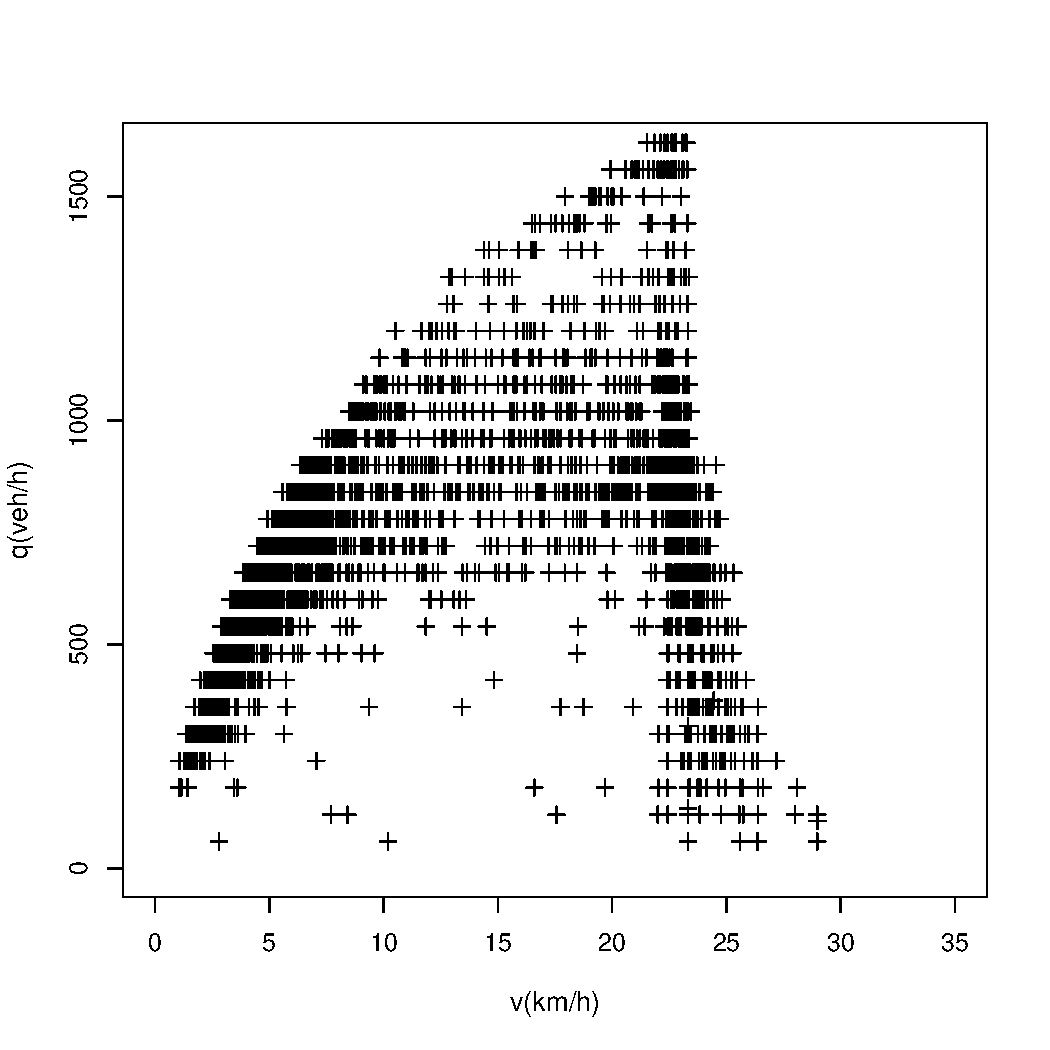
\includegraphics[width=0.33\linewidth]{factor1_vq_per25}}
\subfloat[][]{%
\label{factor1_vq_per50}%
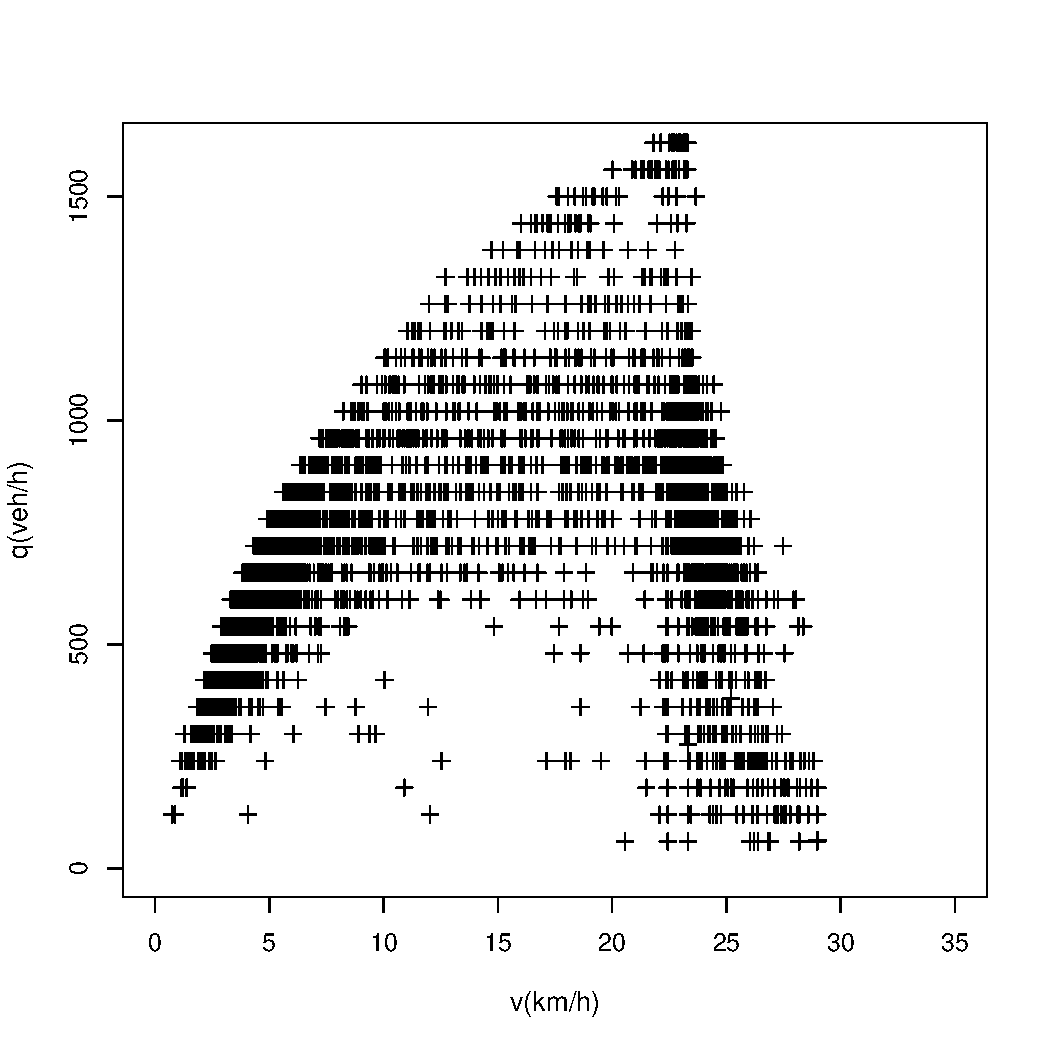
\includegraphics[width=0.33\linewidth]{factor1_vq_per50}}\\%
\subfloat[][]{%
\label{factor1_vq_per75}%
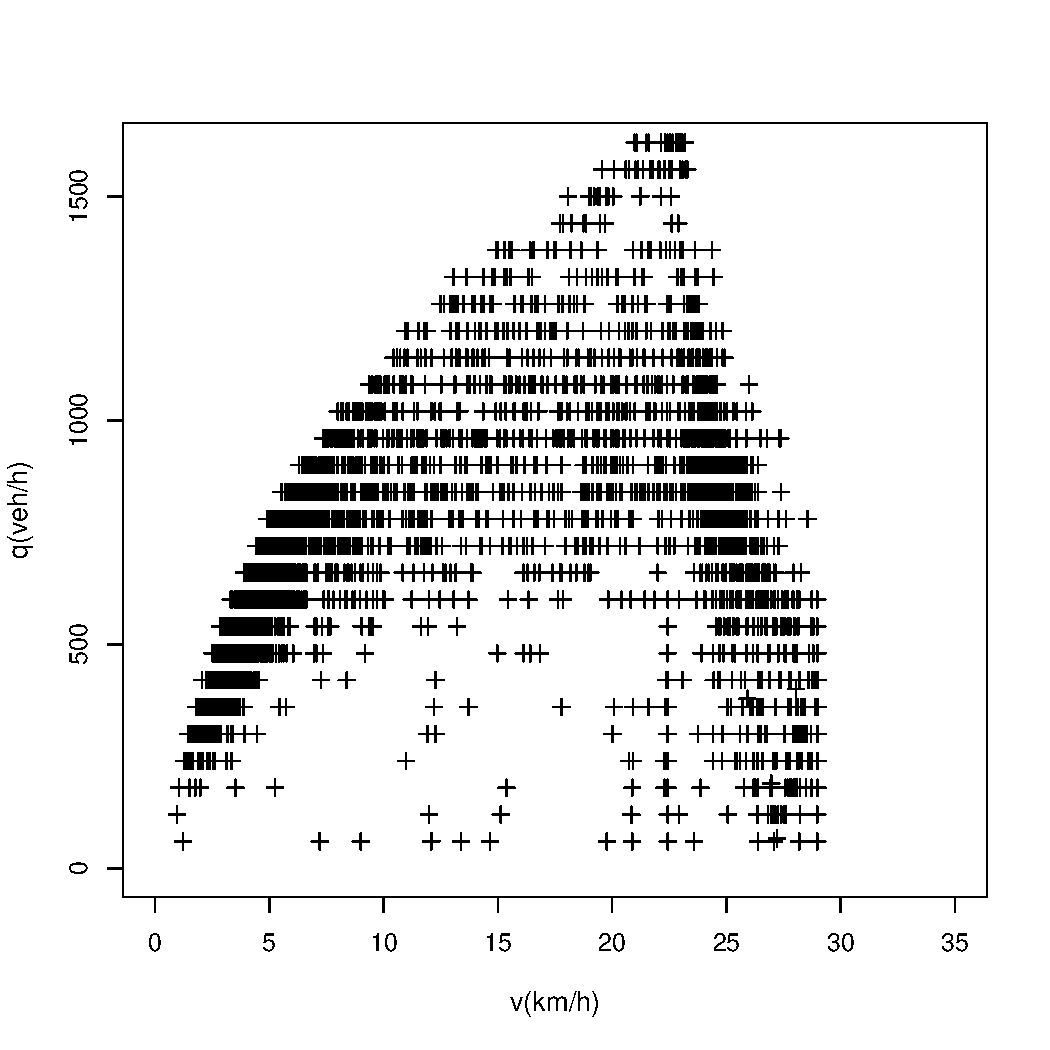
\includegraphics[width=0.33\linewidth]{factor1_vq_per75}}%
\subfloat[][]{%
\label{factor1_vq_per100}%
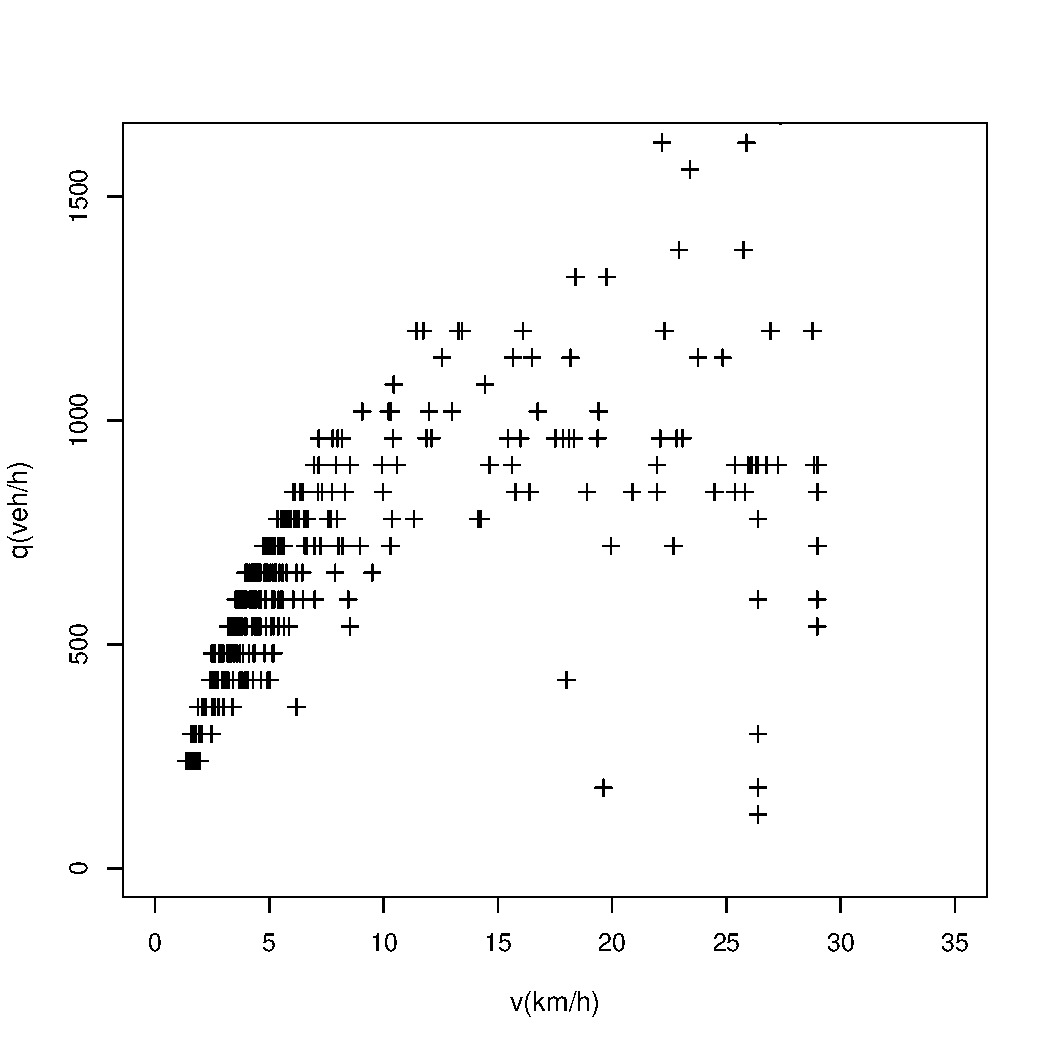
\includegraphics[width=0.33\linewidth]{factor1_vq_per100}}
\caption[A set of four sub-floats.]{期望速度影响下速度流量关系图
\subref{factor1_vq_per0}
\subref{factor1_vq_per25} 
\subref{factor1_vq_per50}
\subref{factor1_vq_per75}
\subref{factor1_vq_per100}分别表示\autoref{speed-factor}中的B型驾驶人的百分比分别为0\%,25\%,50\%,75\%,100\%}%
\label{factor1_vq}%
\end{figure}

由\autoref{factor1_vq}看出,期望速度主要对速度-流量关系图中的形状有影响,对最大通行能力和最大通行能力所对应的最佳车速基本没有影响,图中可以看出最大通行能力约为1600veh/h,最佳速度大约均在22km/h。期望速度对速度-流量关系图中的形状的影响主要体现在,最佳车速的右侧主要为自由流的阶段。由于两组的期望速度均超过了最佳车速,因此不能排除当期望速度低于最佳车速时可能会对最大通行能力产生影响。



\begin{figure}[!htb]%
\centering
\subfloat[][]{
\label{factor1_kq_per0}%
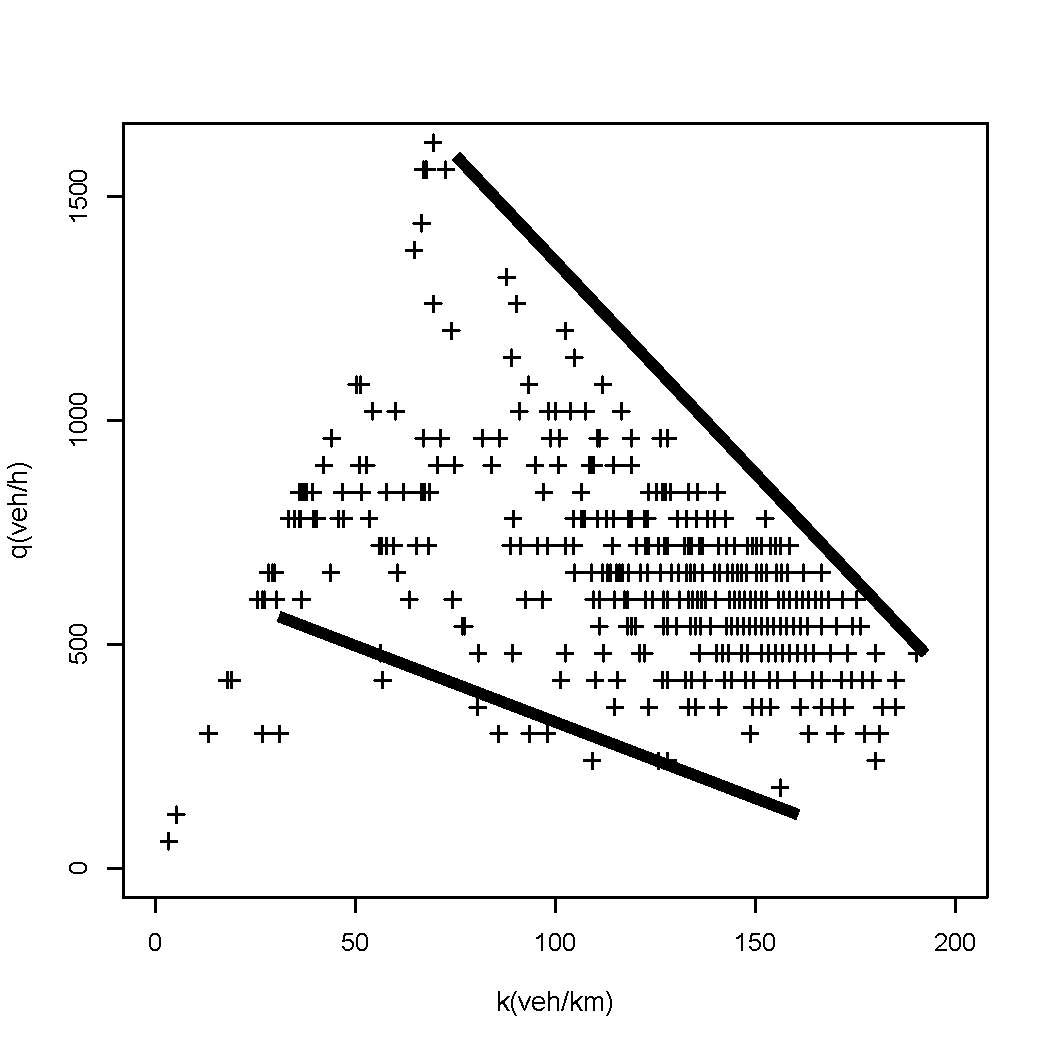
\includegraphics[width=0.33\linewidth]{factor1_kq_per0}
}%
\subfloat[][]{%
\label{factor1_kq_per25}%
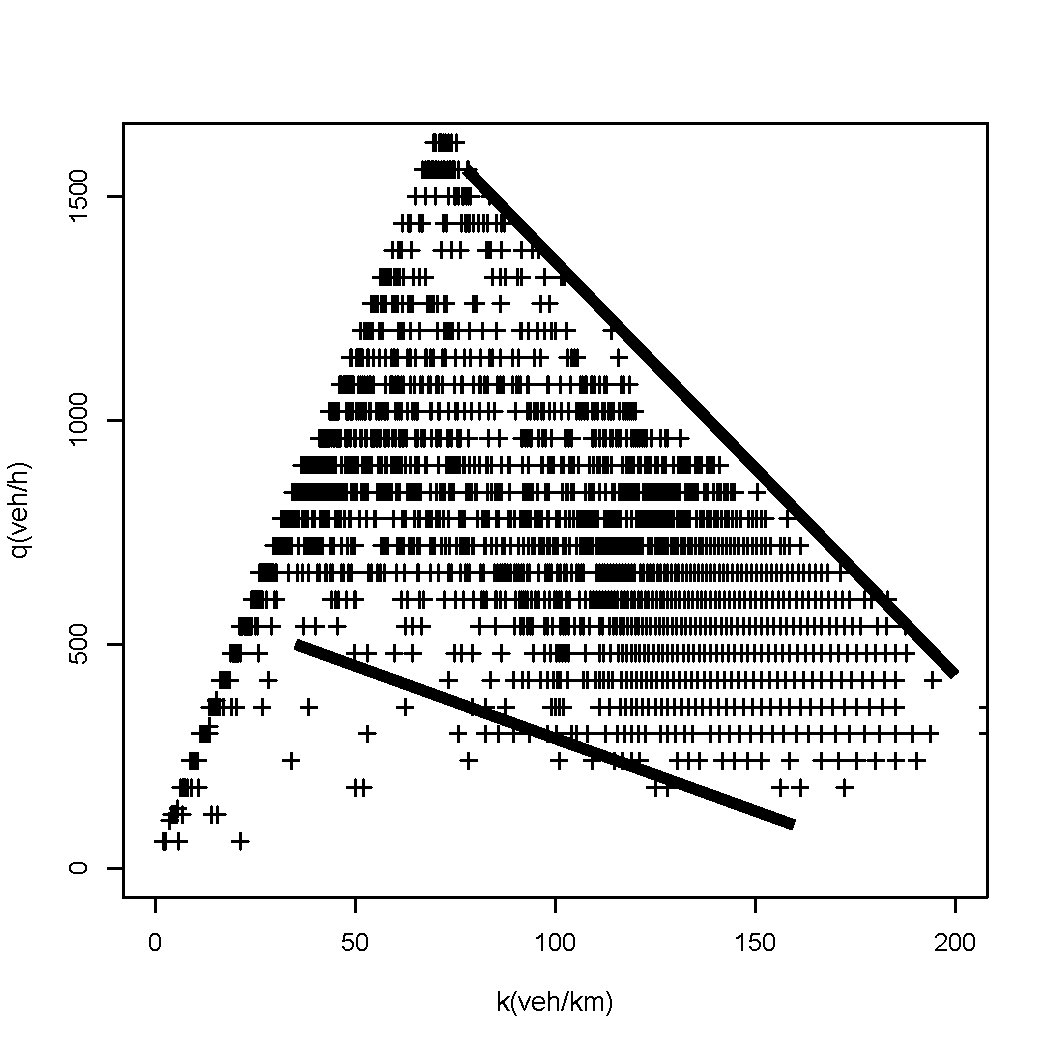
\includegraphics[width=0.33\linewidth]{factor1_kq_per25}}
\subfloat[][]{%
\label{factor1_kq_per50}%
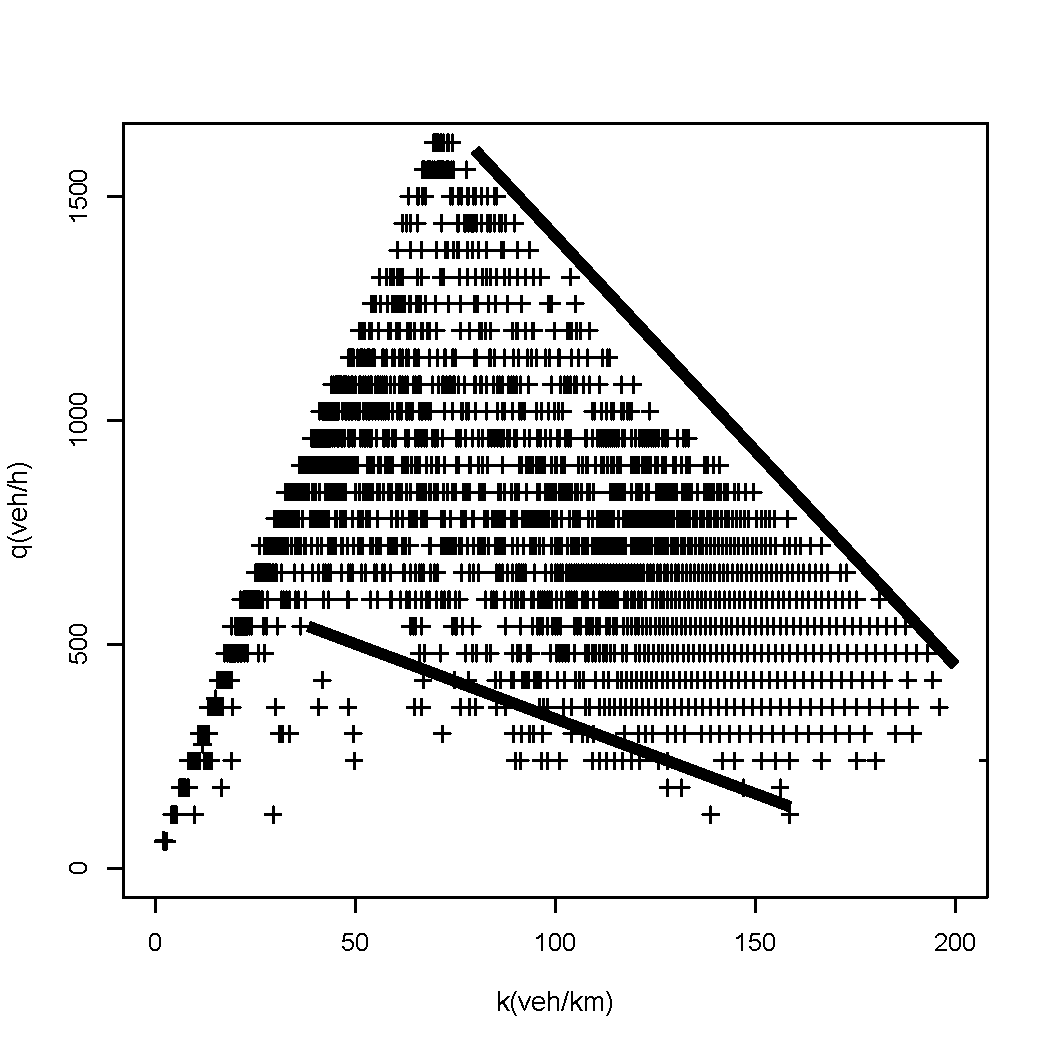
\includegraphics[width=0.33\linewidth]{factor1_kq_per50}}\\%
\subfloat[][]{%
\label{factor1_kq_per75}%
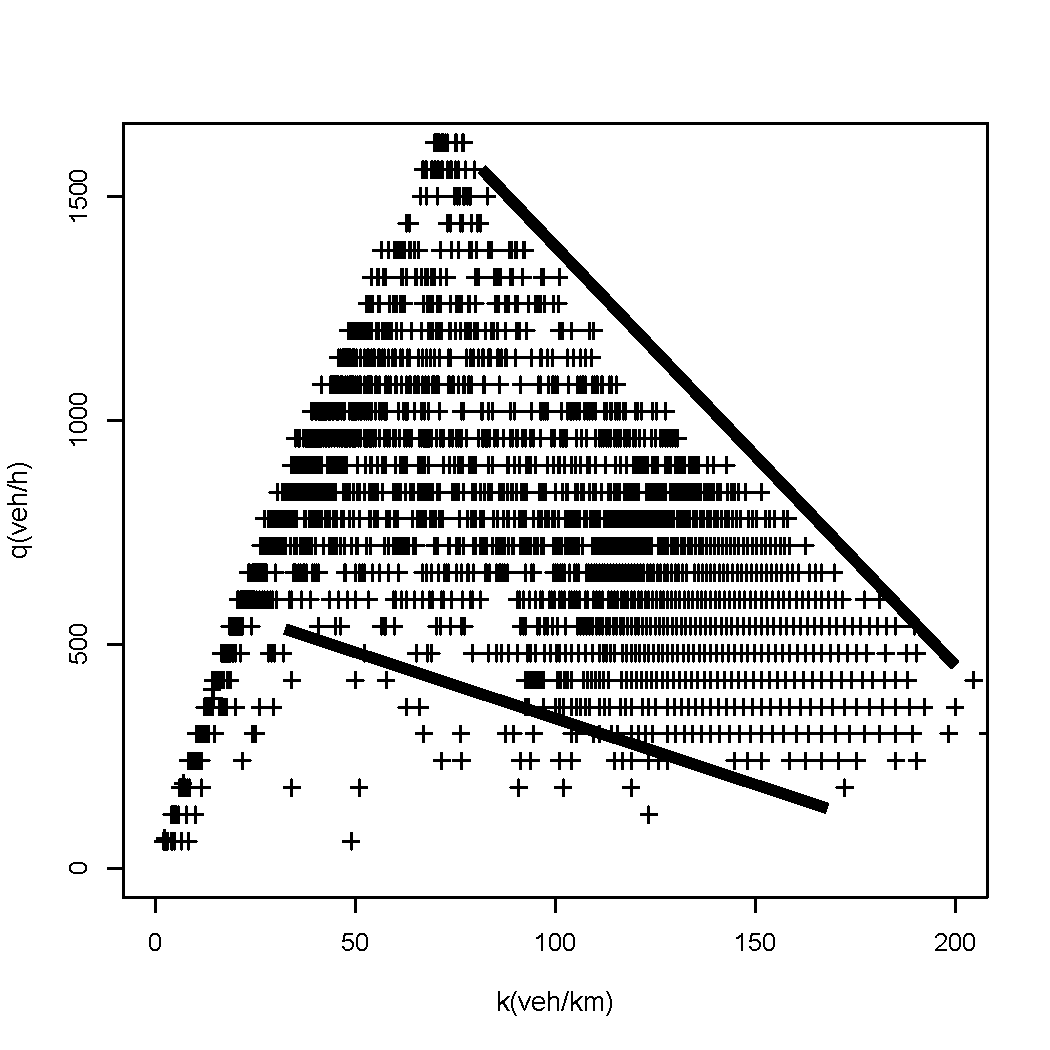
\includegraphics[width=0.33\linewidth]{factor1_kq_per75}}%
\subfloat[][]{%
\label{factor1_kq_per100}%
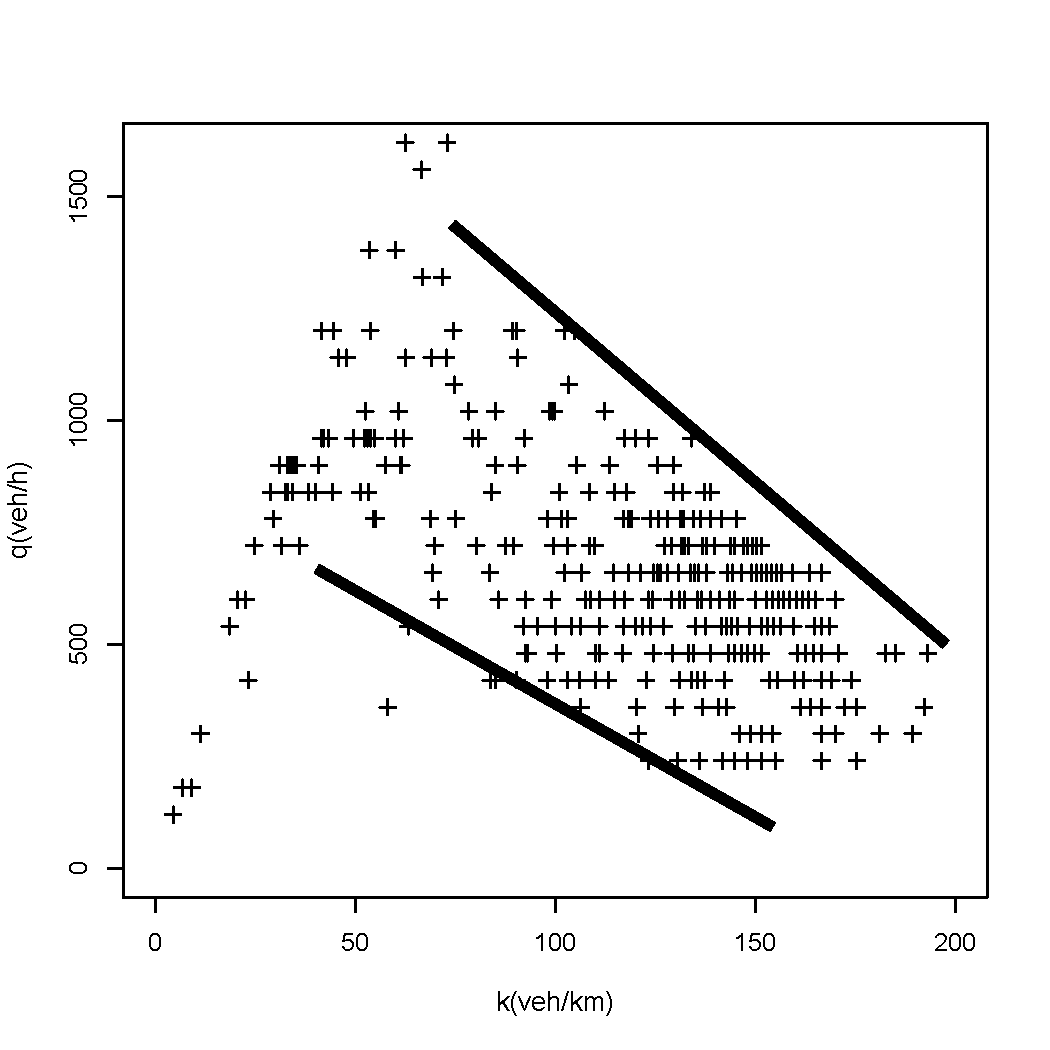
\includegraphics[width=0.33\linewidth]{factor1_kq_per100}}
\caption[A set of four sub-floats.]{期望速度影响下的密度流量关系图
\subref{factor1_kq_per0}
\subref{factor1_kq_per25} 
\subref{factor1_kq_per50}
\subref{factor1_kq_per75}
\subref{factor1_kq_per100}分别表示\autoref{speed-factor}中的B型驾驶人的百分比分别为0\%,25\%,50\%,75\%,100\%}%
\label{factor1_kq}%
\end{figure}

由\autoref{factor1_kq}看,期望速度对最佳密度基本没有影响。根据Kerner的三相交通流理论,道路介于最大和最小通行能力之间具有无数个通行能力,\autoref{factor1_kq}中e的最小通行能力稍大于其他的情况,这似乎表明最小通行能力受到最低期望车速的影响。由于低期望车速的驾驶人的存在,???根据三相交通流中Speed adaptation效用的作用,低速车辆的阻碍造成最低通行能力的下降是可以理解的。

\subsection{最大减速度影响因素}

\begin{figure}[!htb]
\begin{center}
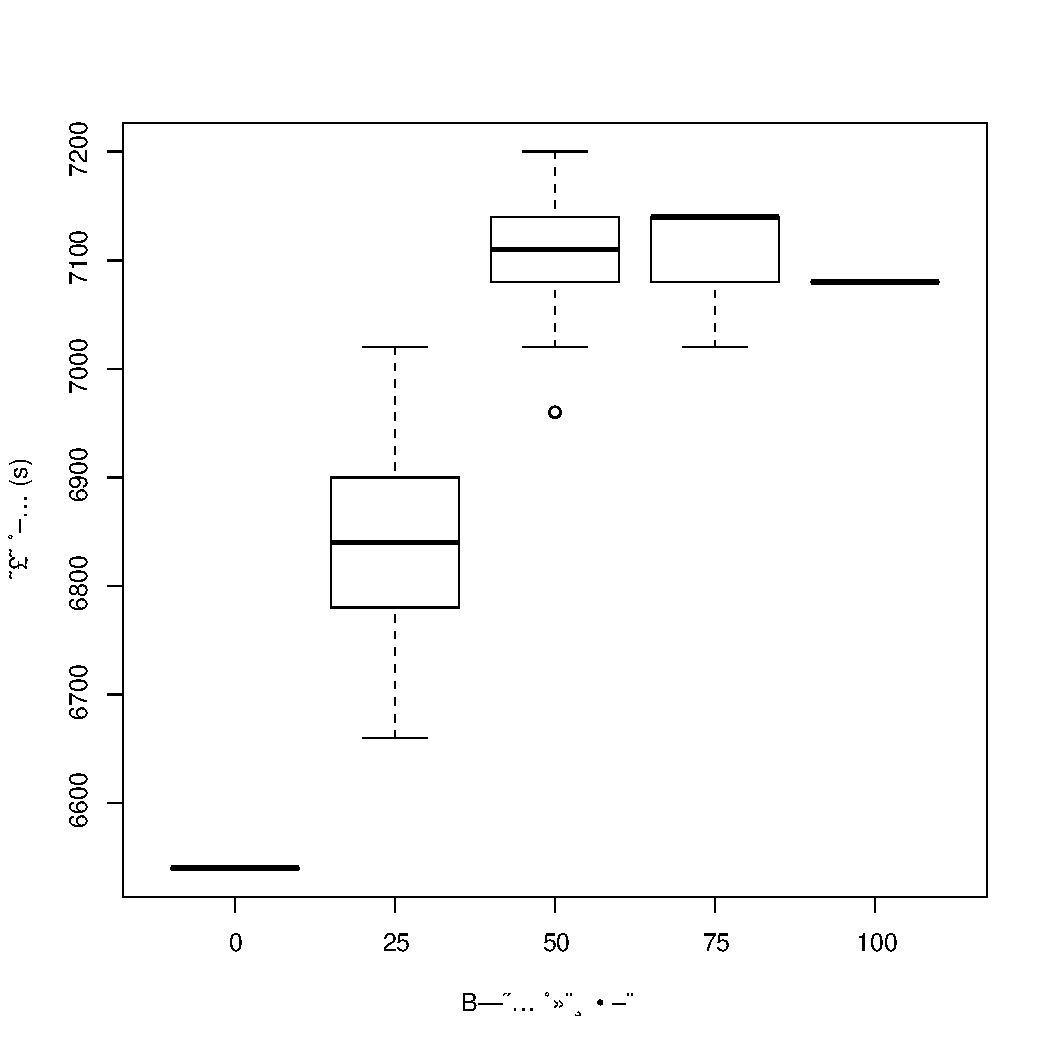
\includegraphics[width=0.5\linewidth]{factor2_box_ttime}
\caption{最大减速度影响下模拟用时箱图}
\label{factor2_box_ttime}
\end{center}
\end{figure}

\autoref{factor2_box_ttime}给出了,期望速度影响下模拟总用时的变化,随着\autoref{decel-factor}中最大减速度较大的B型驾驶人的增加,模拟所用时间呈现上升的趋势。对于单纯类型的驾驶人组合,最大减速度由2.33$m/s^2$增加4.29$m/s^2$,增加84\%,模拟用时从6540s增加到7080s,增加了8.3\%。

少量的B型驾驶人即可对总模拟用时造成较大影响。


\begin{figure}[!htb]%
\centering
\subfloat[][]{
\label{factor2_vq_per0}%
\includegraphics[width=0.33\linewidth]{factor2_vq_per0}
}%
\subfloat[][]{%
\label{factor2_vq_per25}%
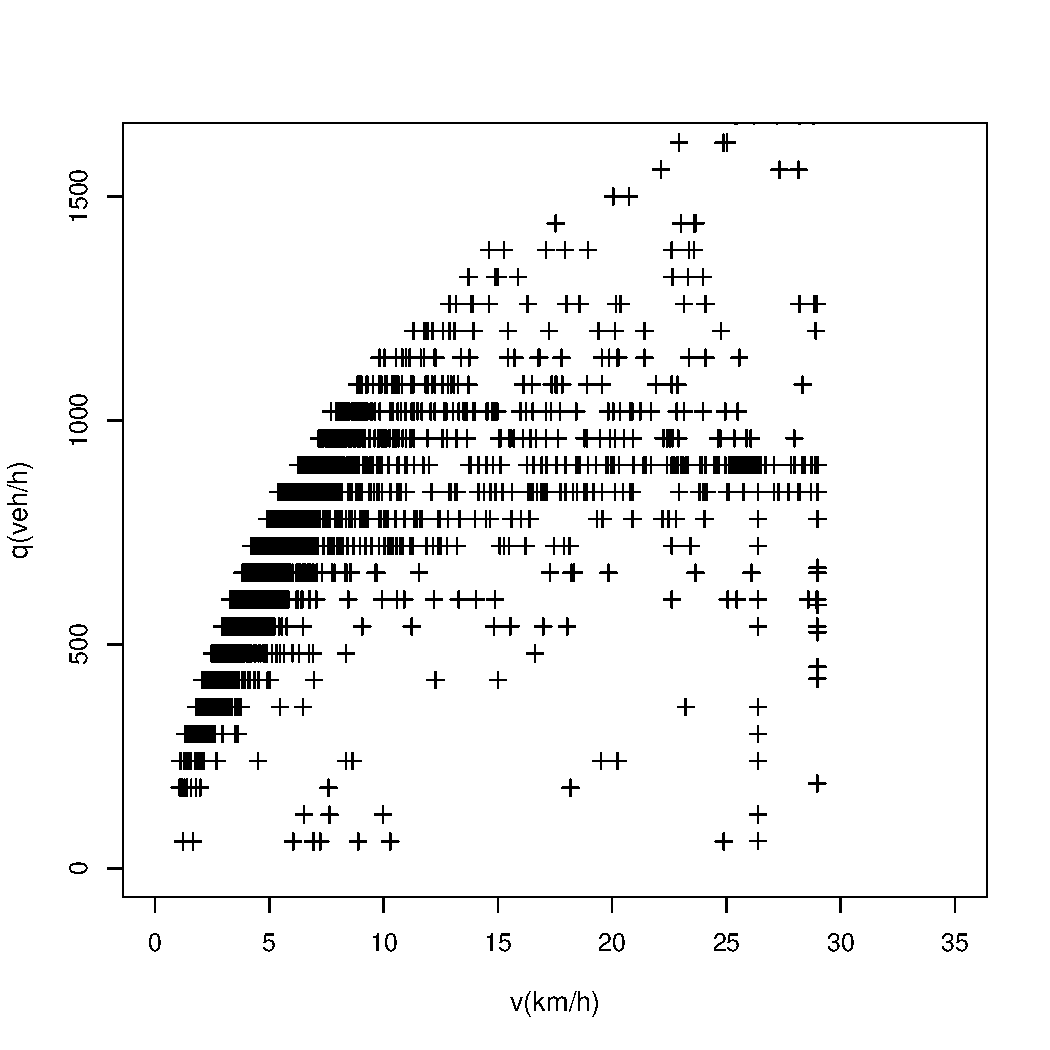
\includegraphics[width=0.33\linewidth]{factor2_vq_per25}}
\subfloat[][]{%
\label{factor2_vq_per50}%
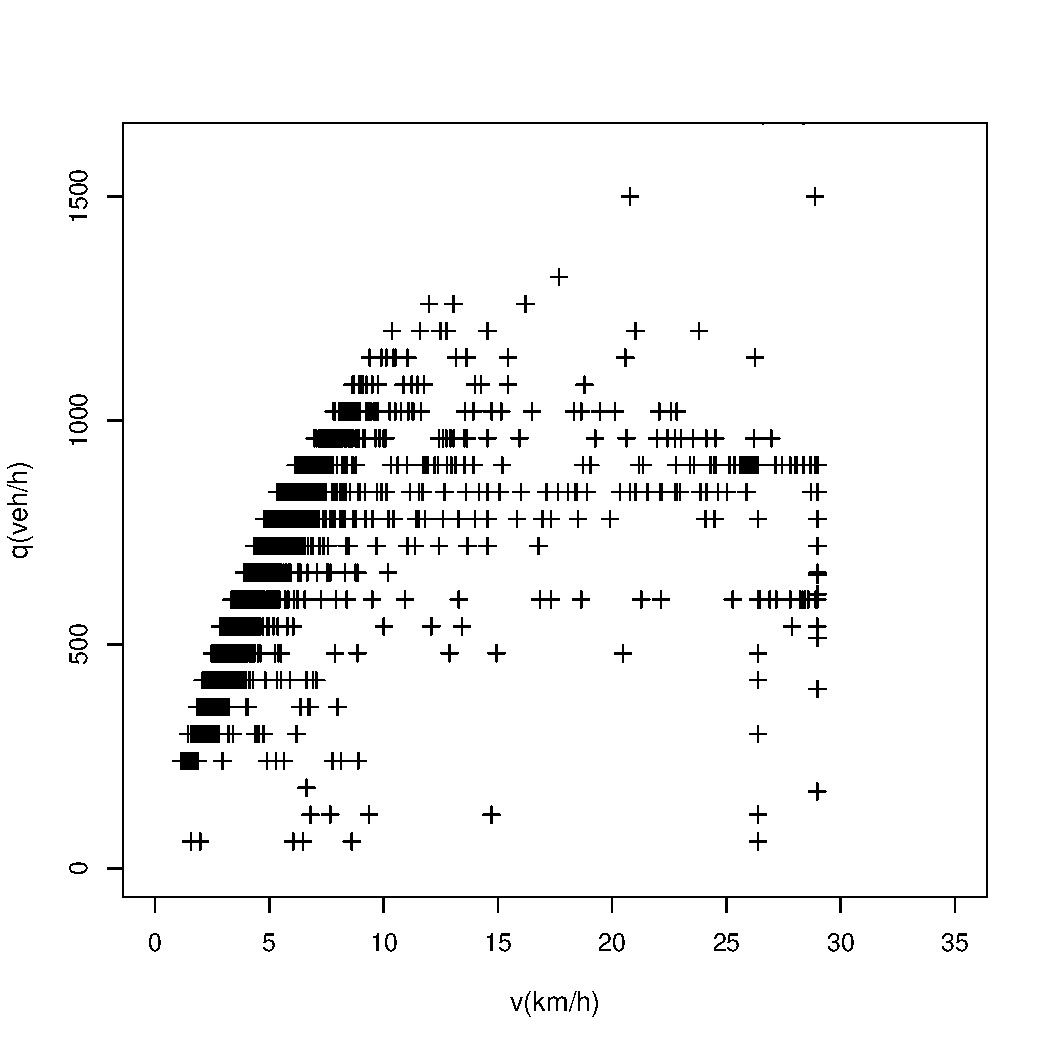
\includegraphics[width=0.33\linewidth]{factor2_vq_per50}}\\%
\subfloat[][]{%
\label{factor2_vq_per75}%
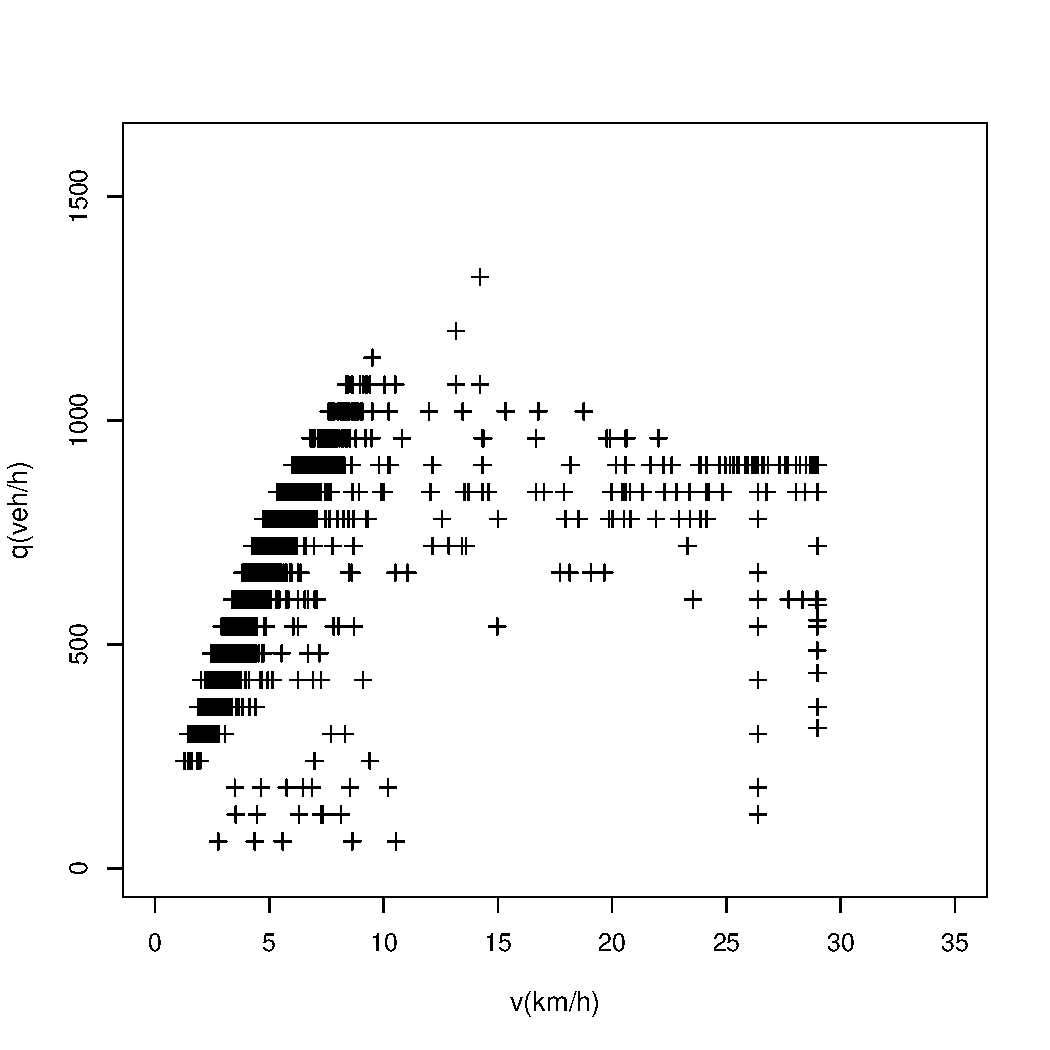
\includegraphics[width=0.33\linewidth]{factor2_vq_per75}}%
\subfloat[][]{%
\label{factor2_vq_per100}%
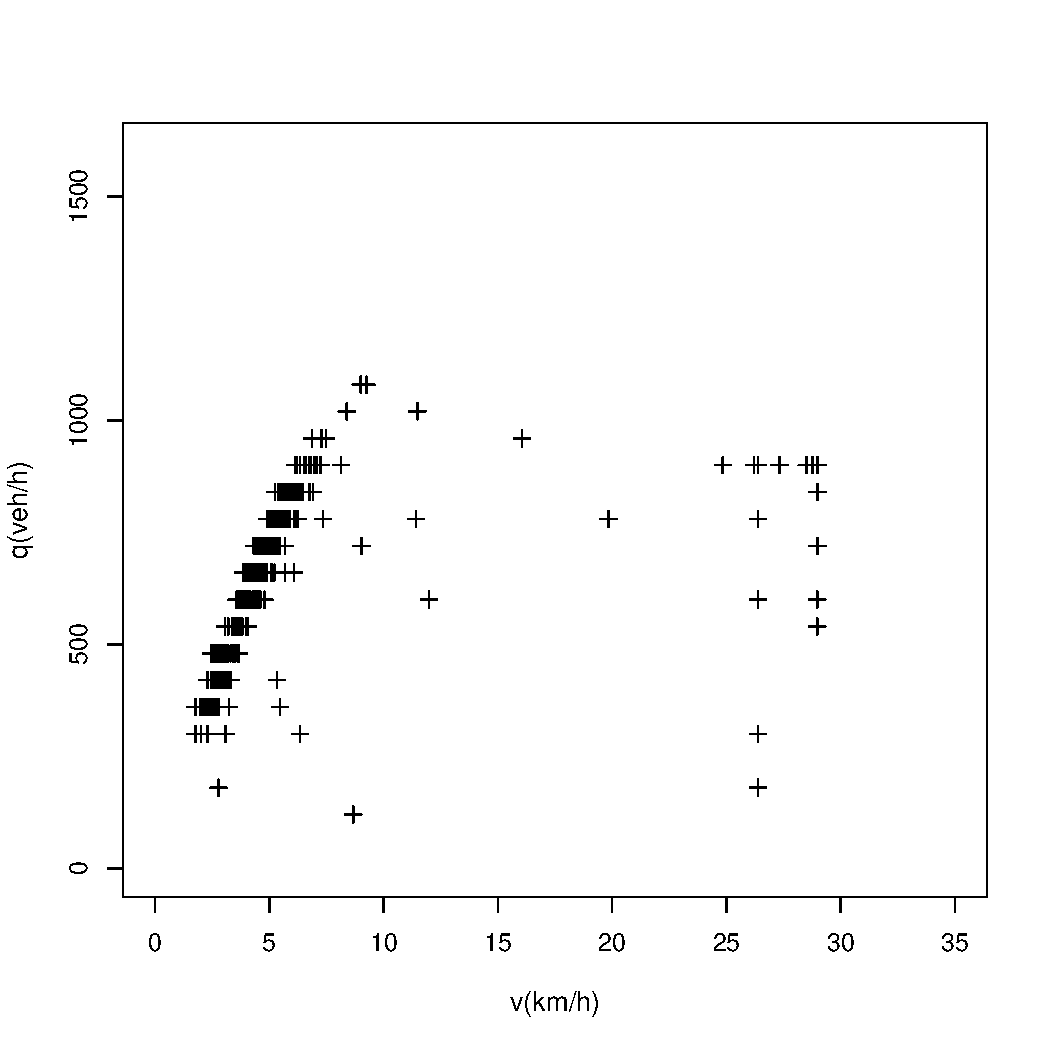
\includegraphics[width=0.33\linewidth]{factor2_vq_per100}}
\caption[A set of four sub-floats.]{最大减速度影响下速度流量关系图
\subref{factor2_vq_per0}
\subref{factor2_vq_per25} 
\subref{factor2_vq_per50}
\subref{factor2_vq_per75}
\subref{factor2_vq_per100}分别表示\autoref{decel-factor}中的B型驾驶人的百分比分别为0\%,25\%,50\%,75\%,100\%}%
\label{factor2_vq}%
\end{figure}



\begin{figure}[!htb]%
\centering
\subfloat[][]{
\label{factor2_kq_per0}%
\includegraphics[width=0.33\linewidth]{factor2_kq_per0}
}%
\subfloat[][]{%
\label{factor2_kq_per25}%
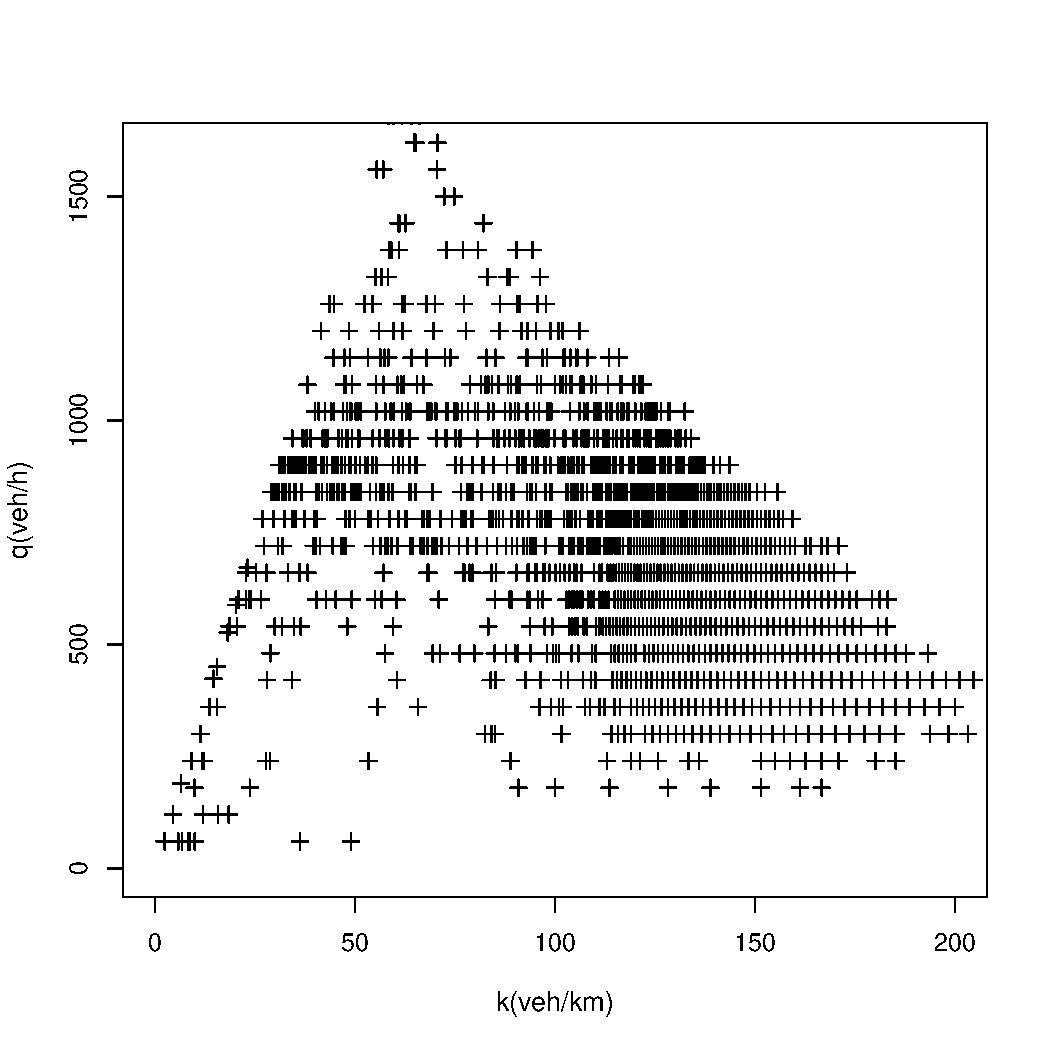
\includegraphics[width=0.33\linewidth]{factor2_kq_per25}}
\subfloat[][]{%
\label{factor2_kq_per50}%
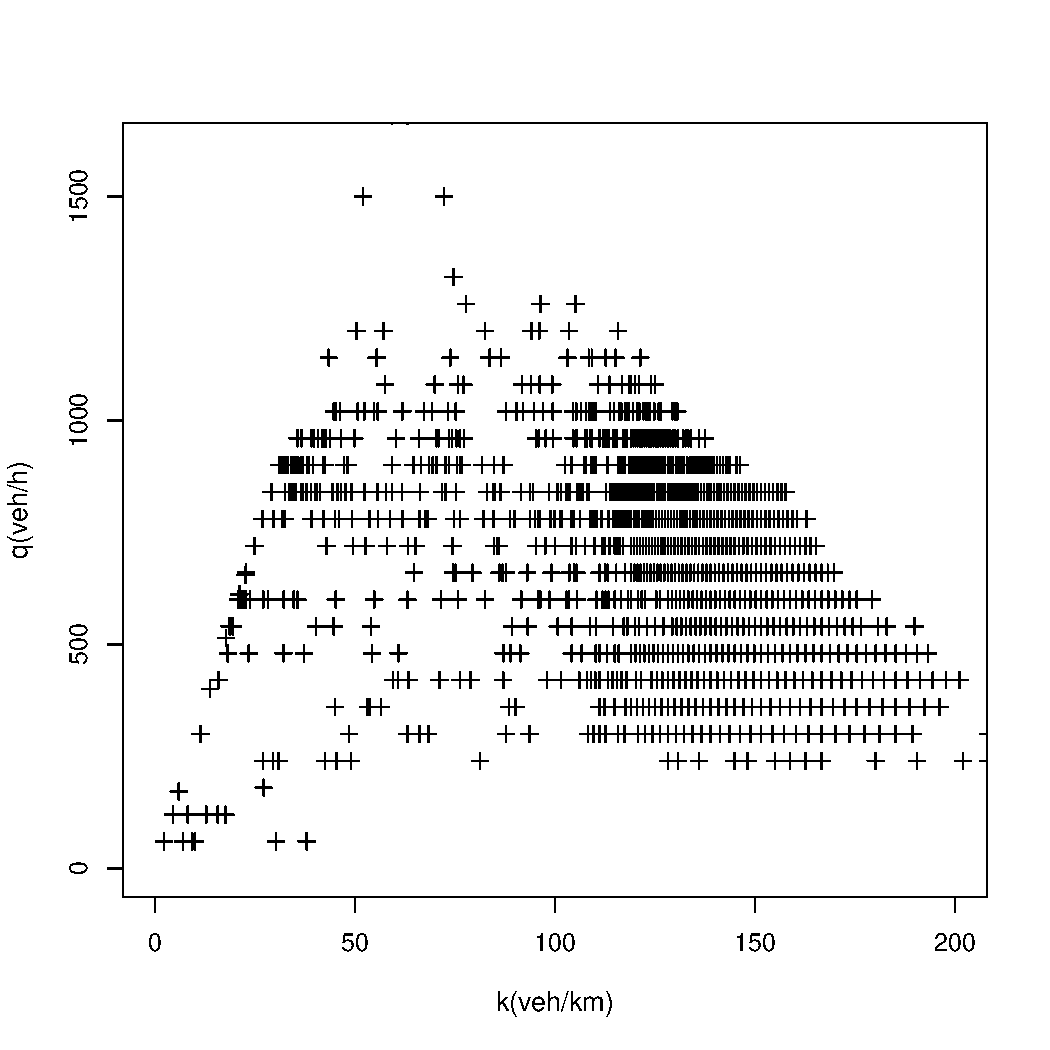
\includegraphics[width=0.33\linewidth]{factor2_kq_per50}}\\%
\subfloat[][]{%
\label{factor2_kq_per75}%
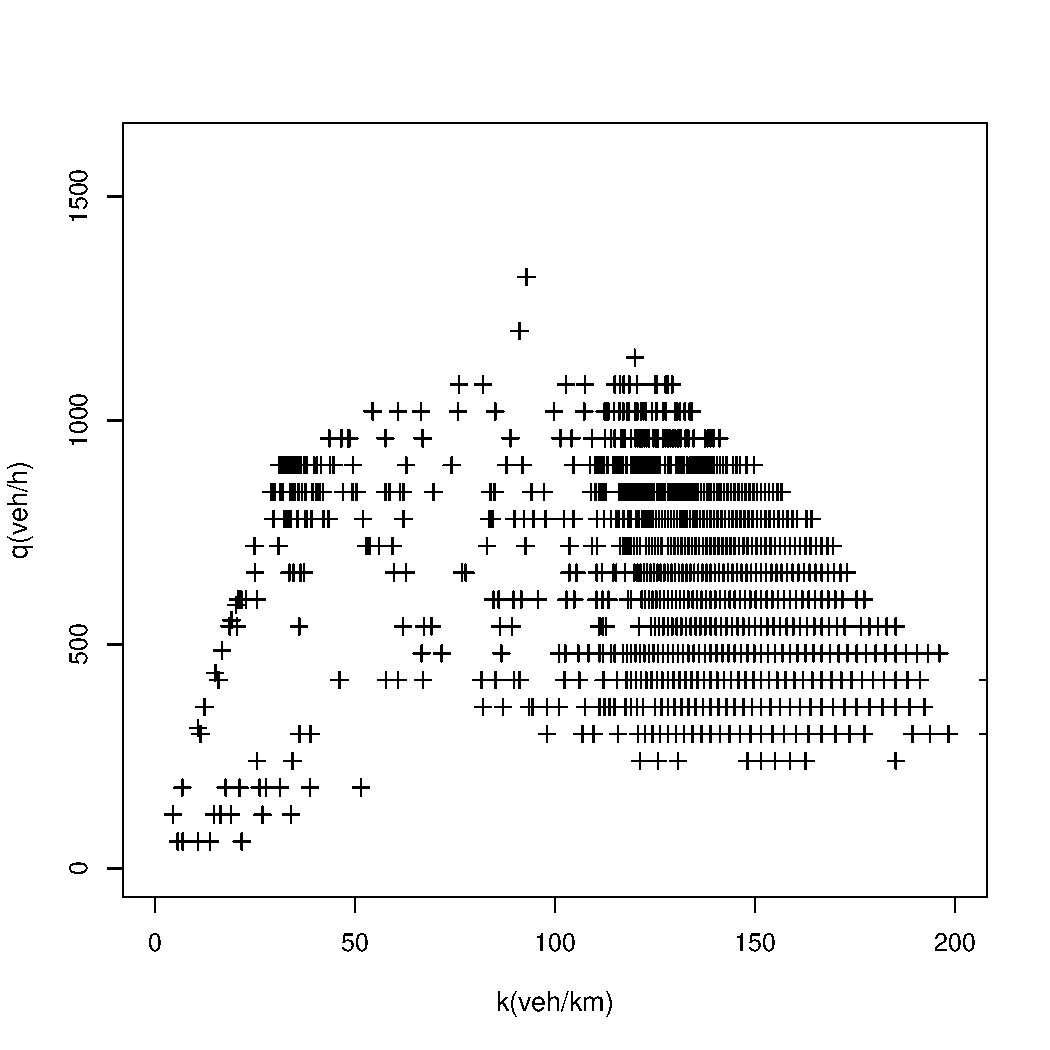
\includegraphics[width=0.33\linewidth]{factor2_kq_per75}}%
\subfloat[][]{%
\label{factor2_kq_per100}%
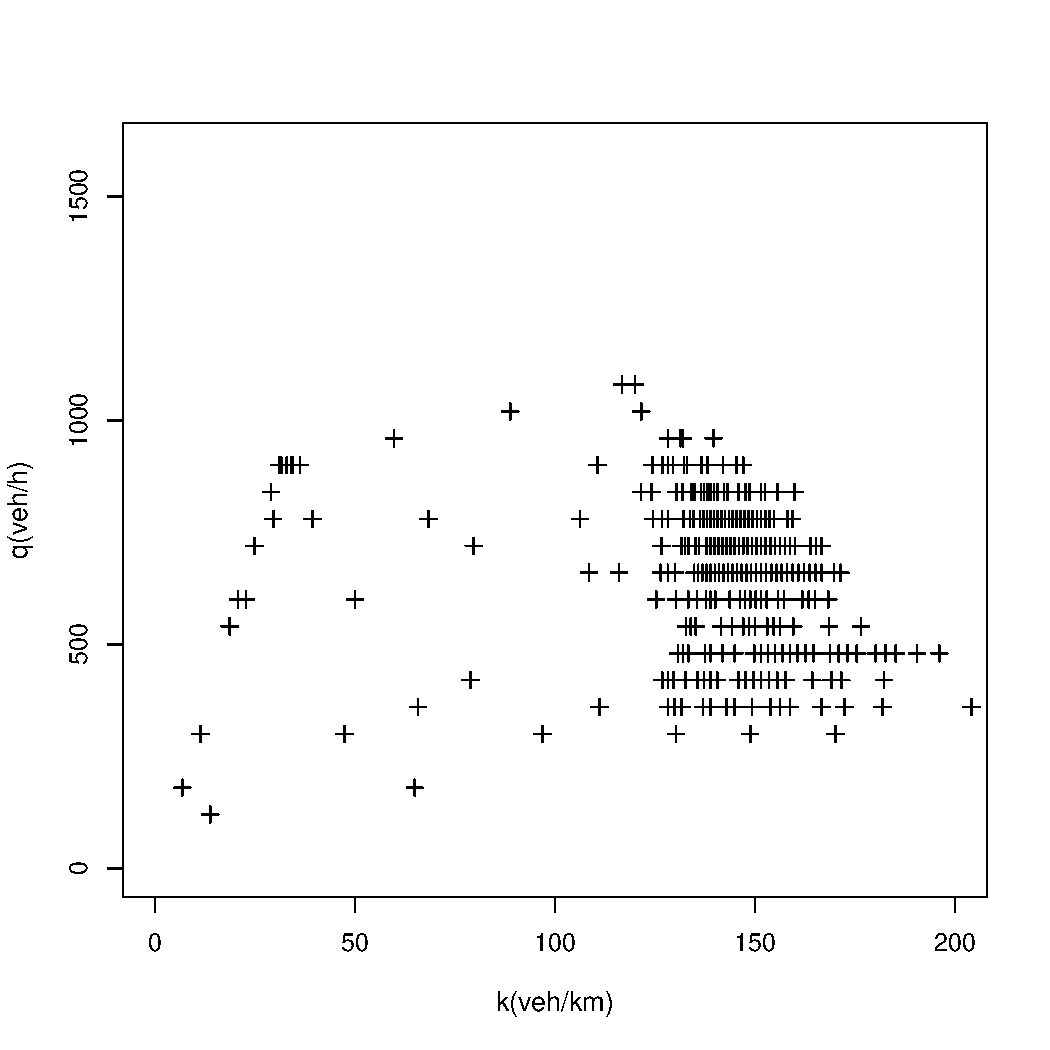
\includegraphics[width=0.33\linewidth]{factor2_kq_per100}}
\caption[A set of four sub-floats.]{最大减速度影响下的密度流量关系图
\subref{factor2_kq_per0}
\subref{factor2_kq_per25} 
\subref{factor2_kq_per50}
\subref{factor2_kq_per75}
\subref{factor2_kq_per100}分别表示\autoref{decel-factor}中的B型驾驶人的百分比分别为0\%,25\%,50\%,75\%,100\%}%
\label{factor2_kq}%
\end{figure}

\autoref{factor2_vq,factor2_kq}给出了,最大减速度影响下速度流量关系图和最大减速度影响下的密度流量关系图,可以看出,随着\autoref{decel-factor}中最大减速度较大的B型驾驶人的比例增加,在速度流量和密度流量关系图上均更难达到最大通行能力。这种趋势随着B型驾驶人的增加而更为明显。



\begin{figure}[!htb]
\begin{center}
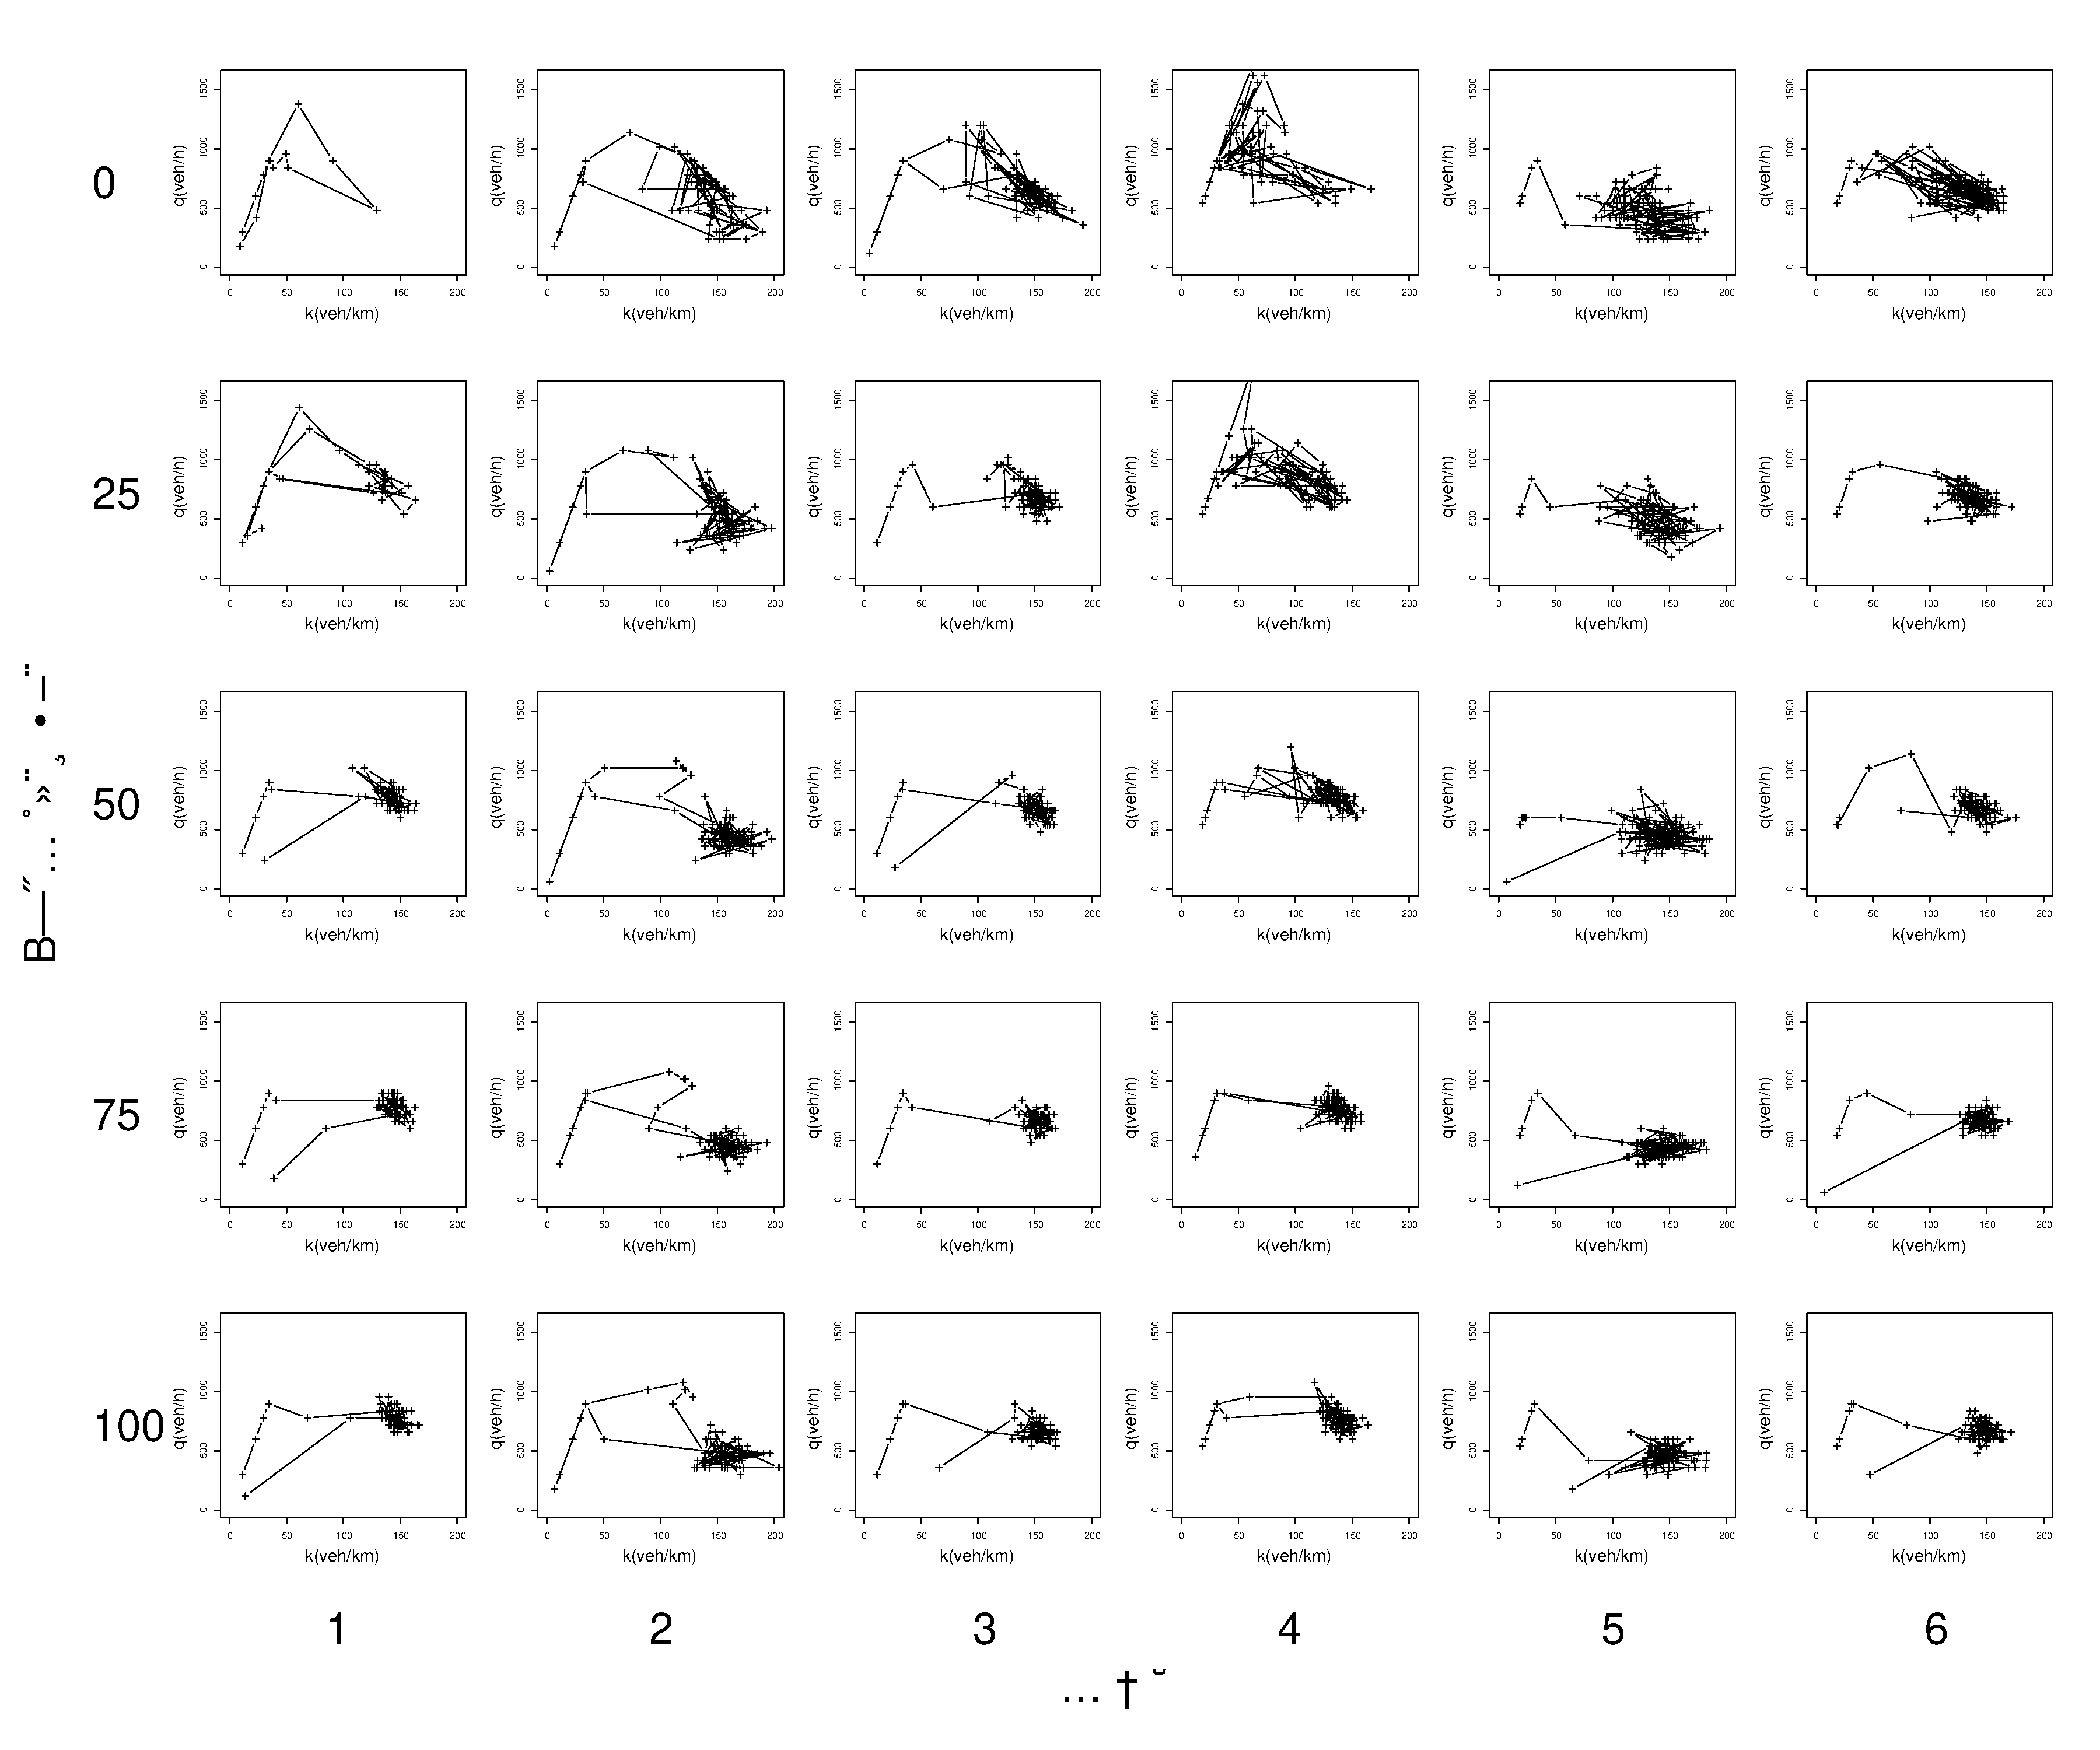
\includegraphics[width=\linewidth]{factor2_kqedges}
\caption{最大减速度影响下各检测器密度流量关系图}
\label{factor2_kqedges}
\end{center}
\end{figure}

最大减速度的增加造成密度流量图上,集中在J线以上,相对不稳定的状态。\autoref{factor2_kqedges}给出了最大减速度影响下各检测器密度流量关系图,从各检测器的密度流量状态跃迁图看,最为明显的是,检测器1和4的最大或接近最大通行能力,随着B型驾驶人的更多的混入,从自由流的状态更多的往同步流状态跃迁。


\subsection{混合影响因素}

\autoref{combined_box_ttime}\autoref{combined_vq}\autoref{combined_kq}\autoref{combined_kqedges},分别给出了混合作用影响下模拟用时箱图,速度流量关系图,密度流量关系图和各检测器密度流量关系图。其结果与最大减速度影响下的结果相似,可以推断对交通流斜率新的影响,主要的贡献成分来自于最大减速度的影响,最大减速度越大则交通流越难达到最大通行能力,也越多的处于较为不稳定的同步流状态。

\begin{figure}[!htb]
\begin{center}
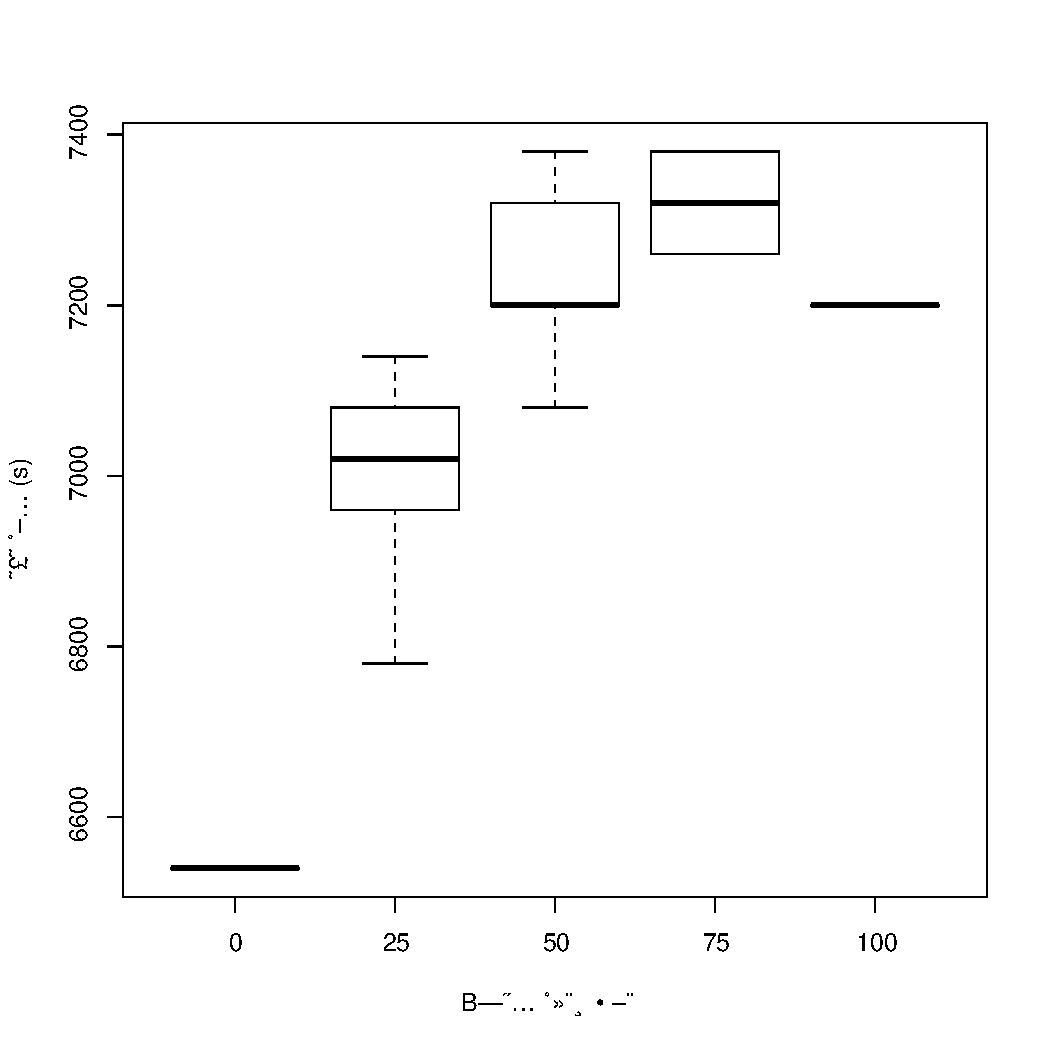
\includegraphics[width=0.5\linewidth]{combined_box_ttime}
\label{combined_box_ttime}
\caption{混合作用影响下模拟用时箱图}
\end{center}
\end{figure}



\begin{figure}[!htb]%
\centering
\subfloat[][]{
\label{combined_vq_per0}%
\includegraphics[width=0.33\linewidth]{combined_vq_per0}
}%
\subfloat[][]{%
\label{combined_vq_per25}%
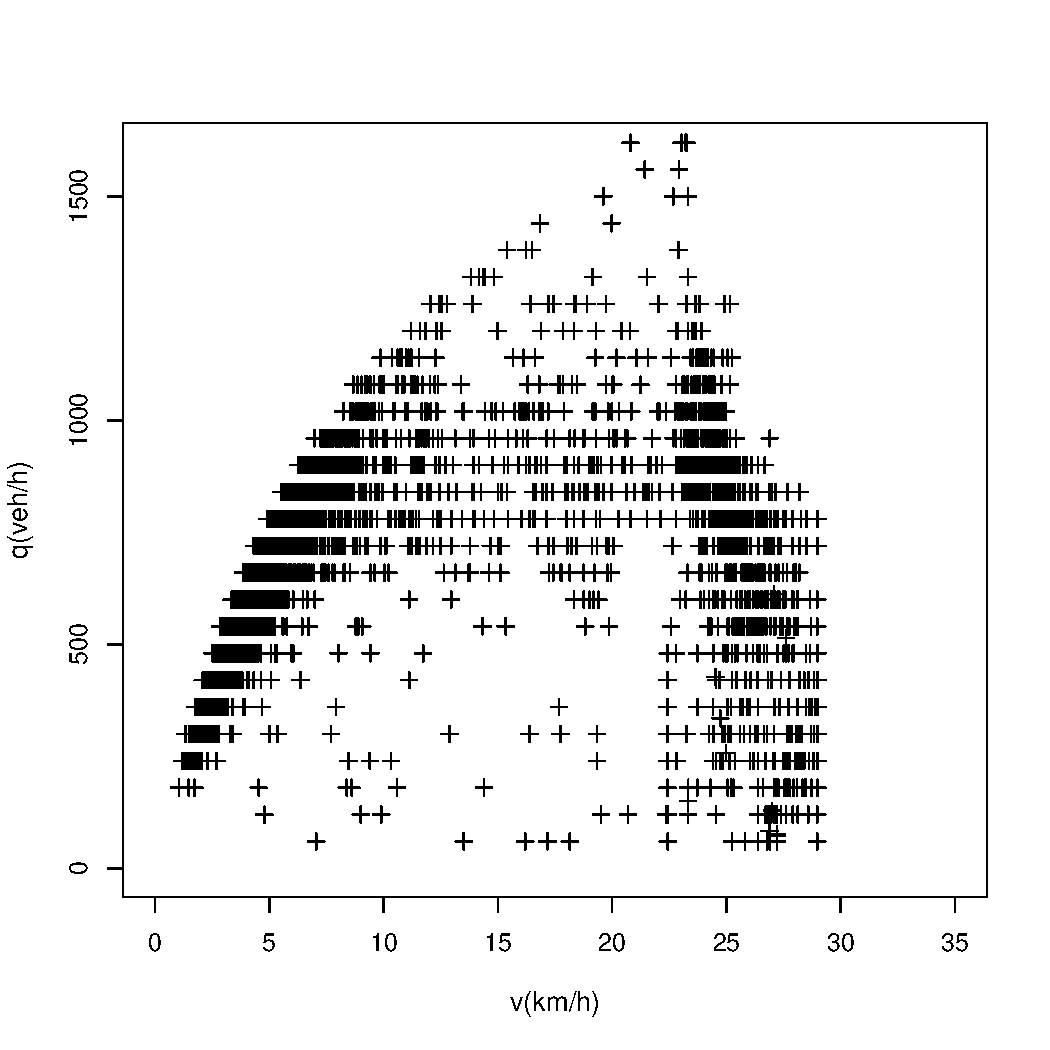
\includegraphics[width=0.33\linewidth]{combined_vq_per25}}
\subfloat[][]{%
\label{combined_vq_per50}%
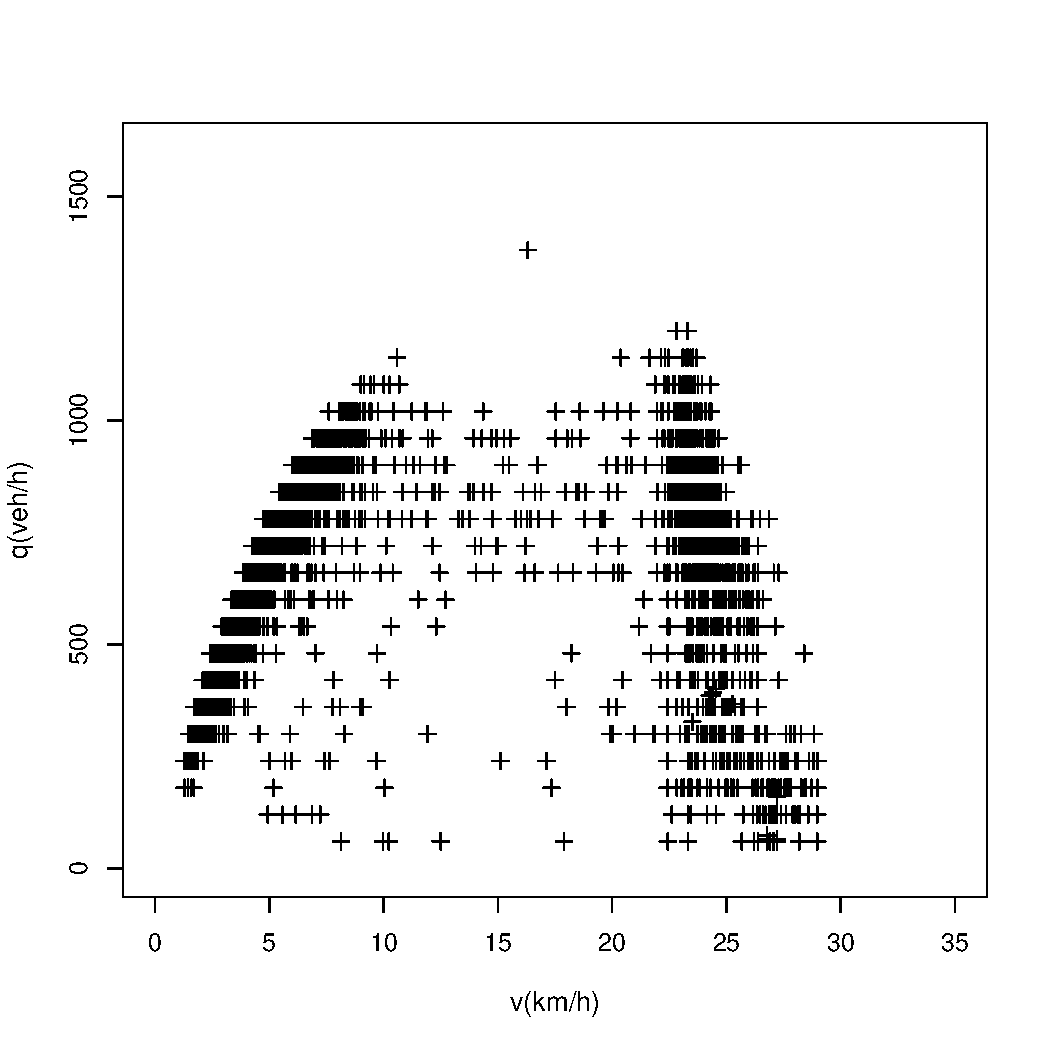
\includegraphics[width=0.33\linewidth]{combined_vq_per50}}\\%
\subfloat[][]{%
\label{combined_vq_per75}%
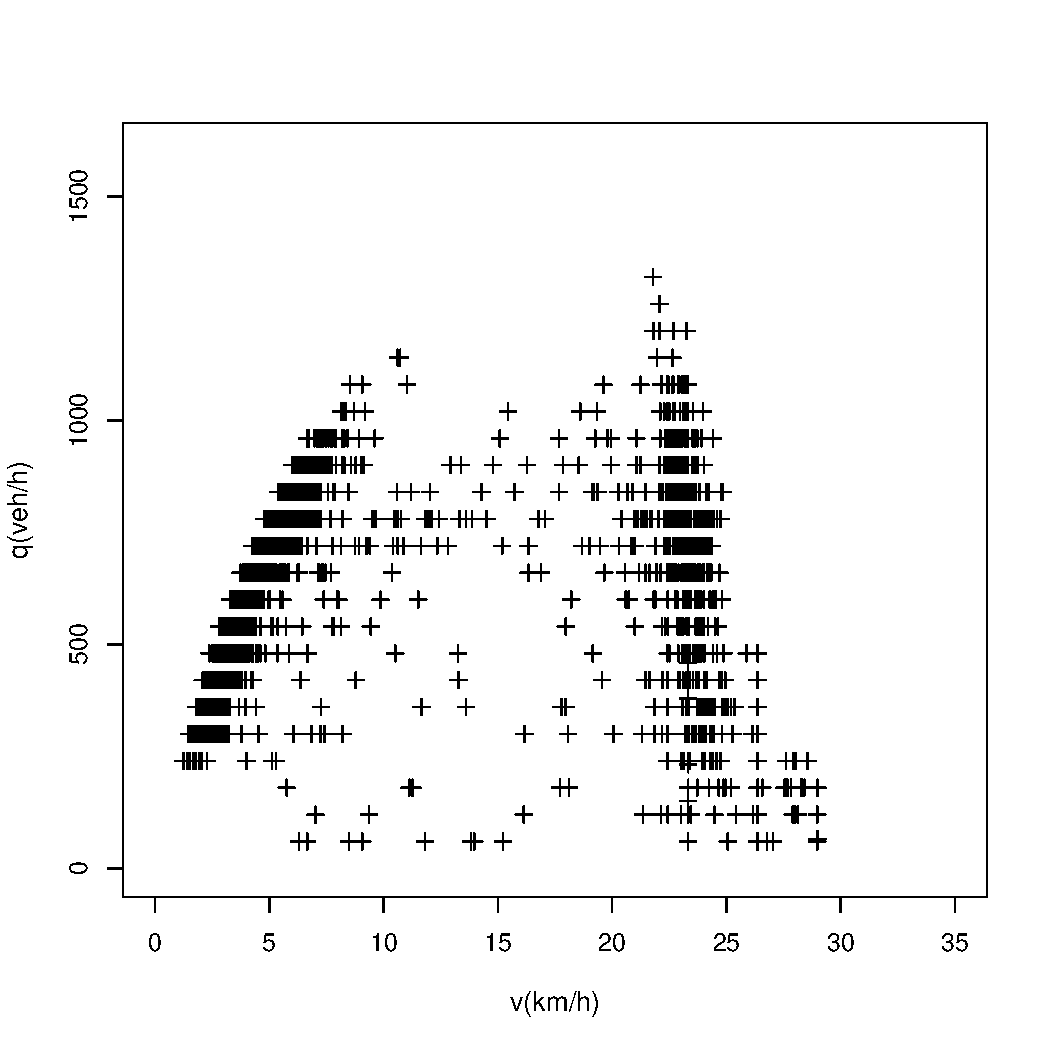
\includegraphics[width=0.33\linewidth]{combined_vq_per75}}%
\subfloat[][]{%
\label{combined_vq_per100}%
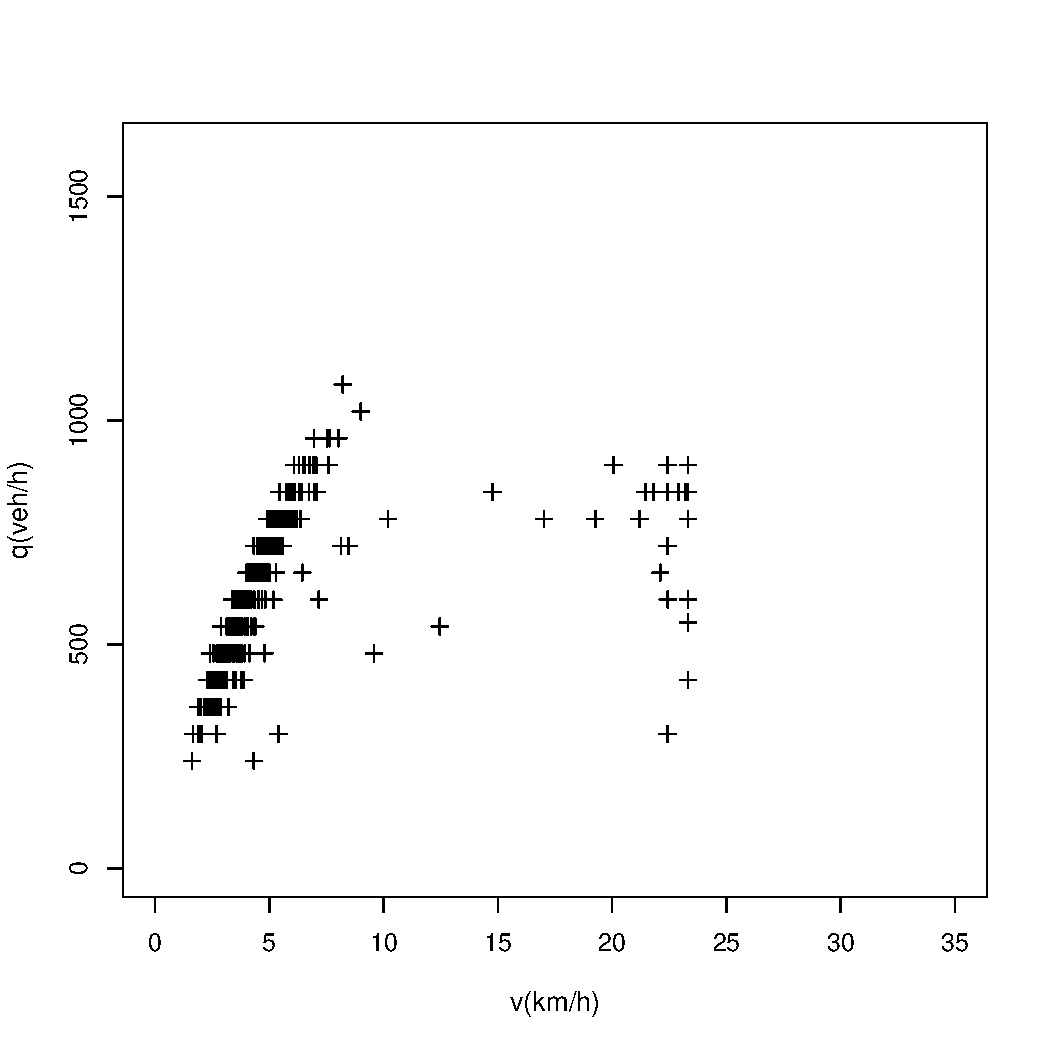
\includegraphics[width=0.33\linewidth]{combined_vq_per100}}
\caption[A set of four sub-floats.]{混合作用影响下速度流量关系图
\subref{combined_vq_per0}
\subref{combined_vq_per25} 
\subref{combined_vq_per50}
\subref{combined_vq_per75}
\subref{combined_vq_per100}分别表示\autoref{combined-factor}中的B型驾驶人的百分比分别为0\%,25\%,50\%,75\%,100\%}%
\label{combined_vq}%
\end{figure}


\begin{figure}[!htb]%
\centering
\subfloat[][]{
\label{combined_kq_per0}%
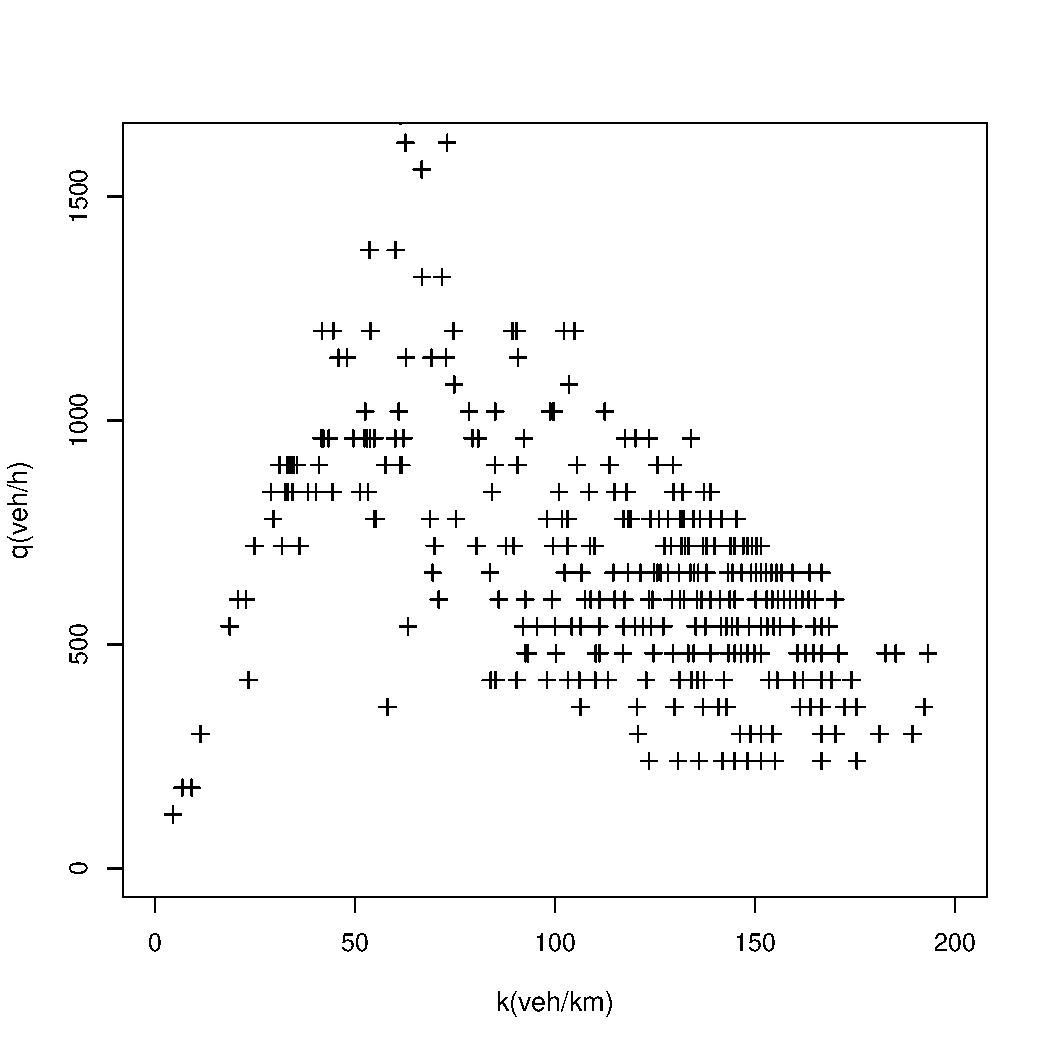
\includegraphics[width=0.33\linewidth]{combined_kq_per0}
}%
\subfloat[][]{%
\label{combined_kq_per25}%
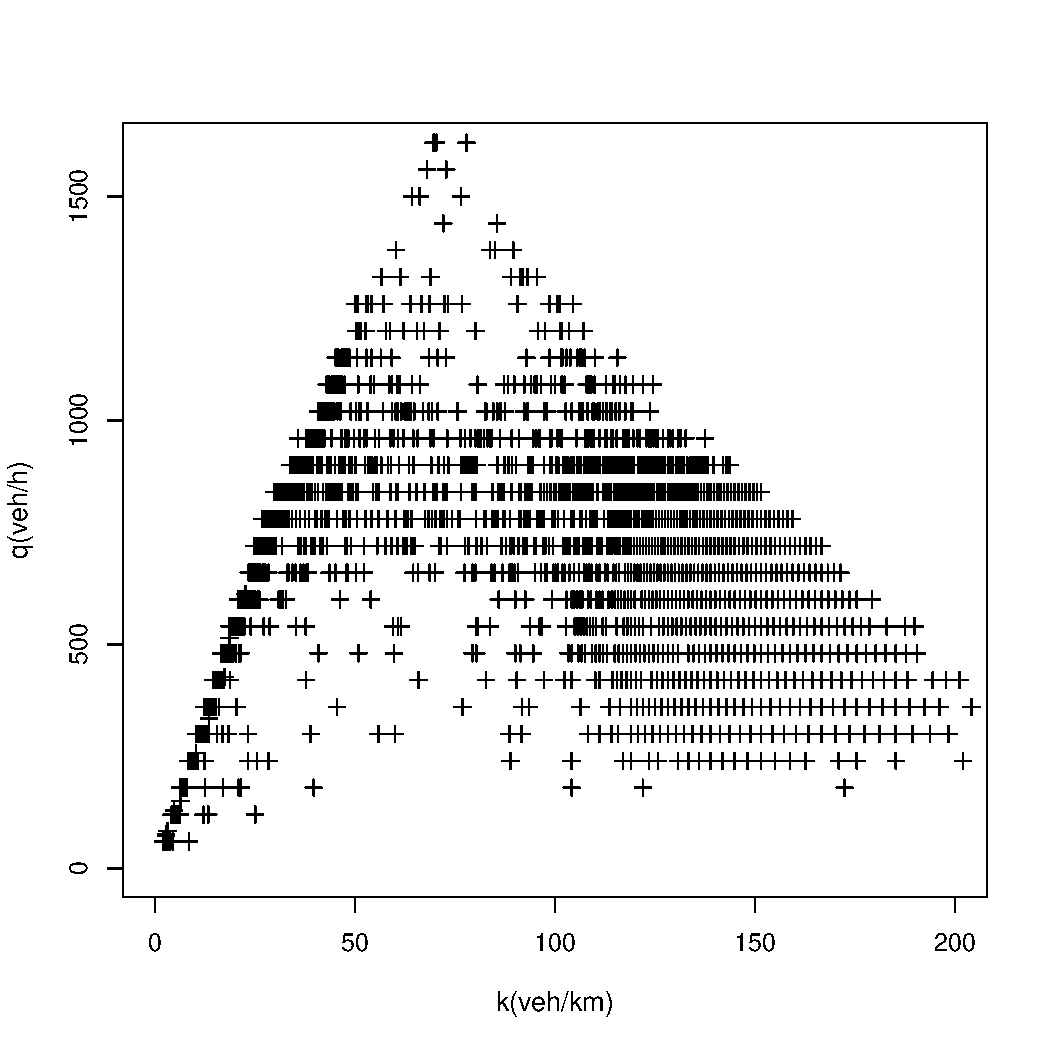
\includegraphics[width=0.33\linewidth]{combined_kq_per25}}
\subfloat[][]{%
\label{combined_kq_per50}%
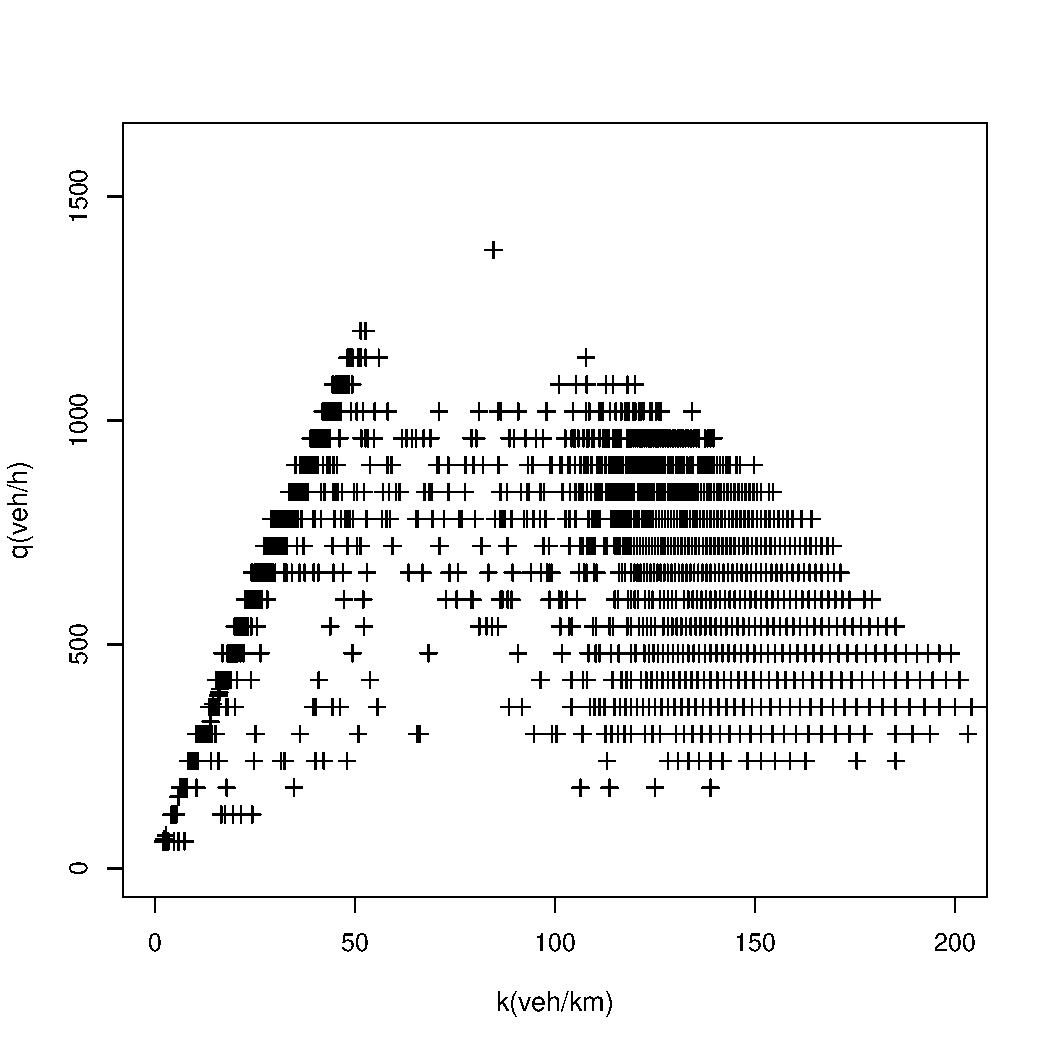
\includegraphics[width=0.33\linewidth]{combined_kq_per50}}\\%
\subfloat[][]{%
\label{combined_kq_per75}%
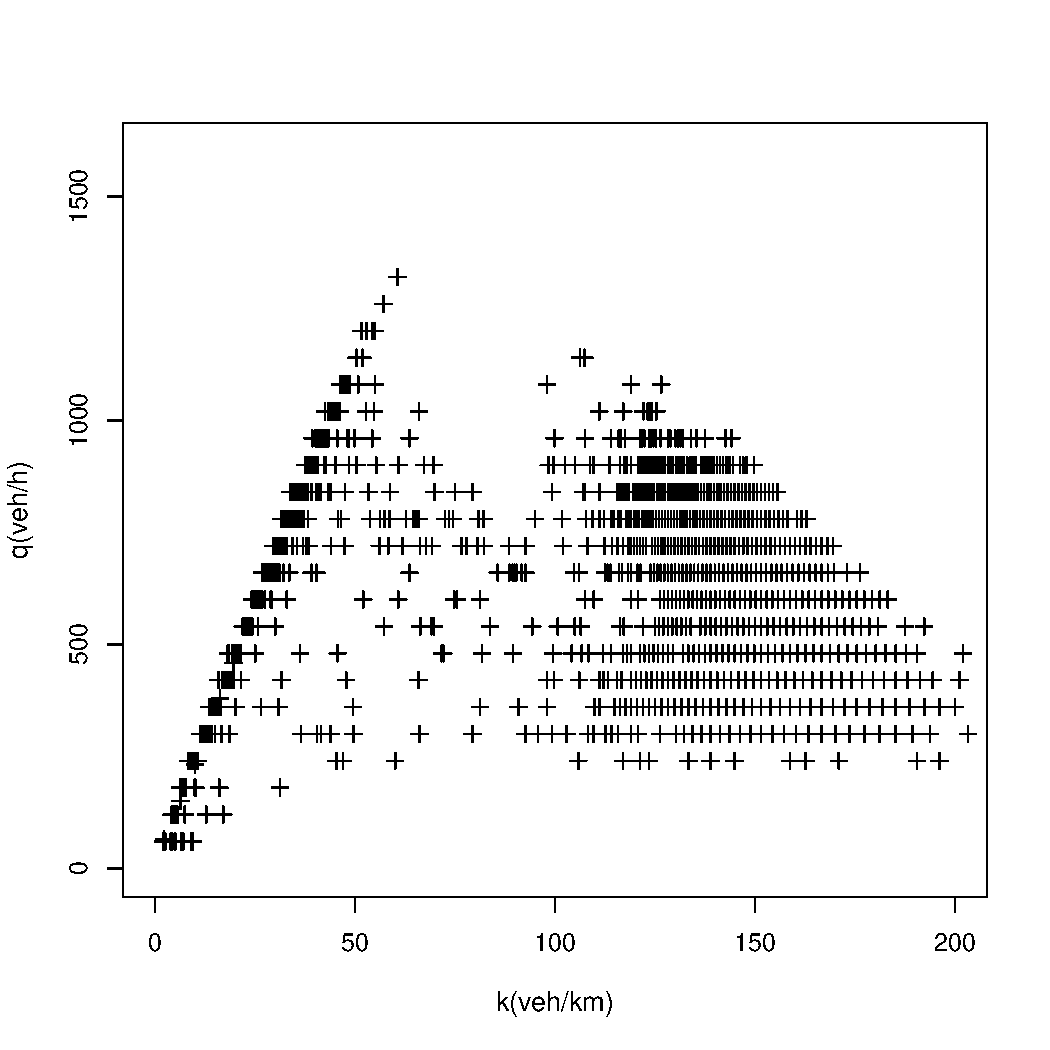
\includegraphics[width=0.33\linewidth]{combined_kq_per75}}%
\subfloat[][]{%
\label{combined_kq_per100}%
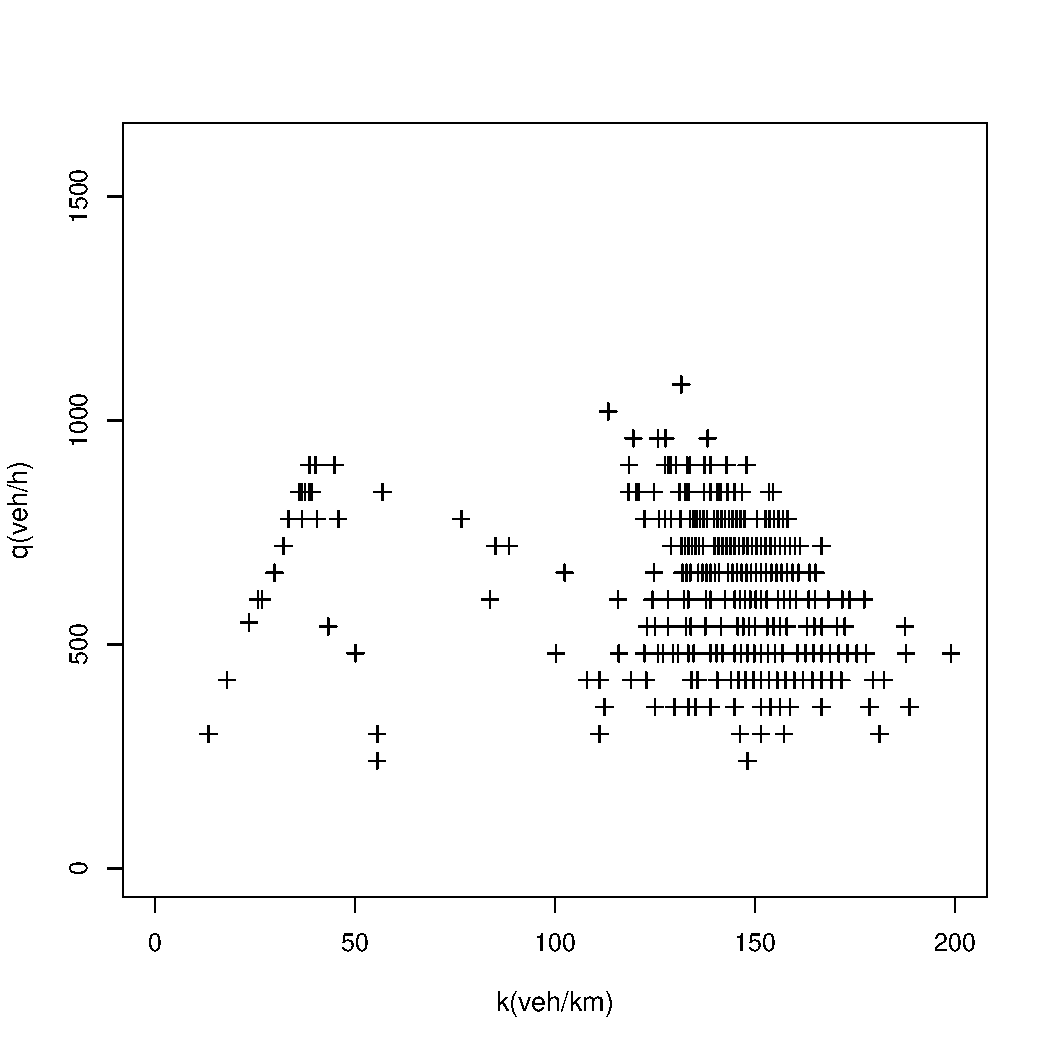
\includegraphics[width=0.33\linewidth]{combined_kq_per100}}
\caption[A set of four sub-floats.]{混合作用影响下的密度流量关系图
\subref{combined_kq_per0}
\subref{combined_kq_per25} 
\subref{combined_kq_per50}
\subref{combined_kq_per75}
\subref{combined_kq_per100}分别表示\autoref{combined-factor}中的B型驾驶人的百分比分别为0\%,25\%,50\%,75\%,100\%}%
\label{combined_kq}%
\end{figure}

\begin{figure}[!htb]
\begin{center}
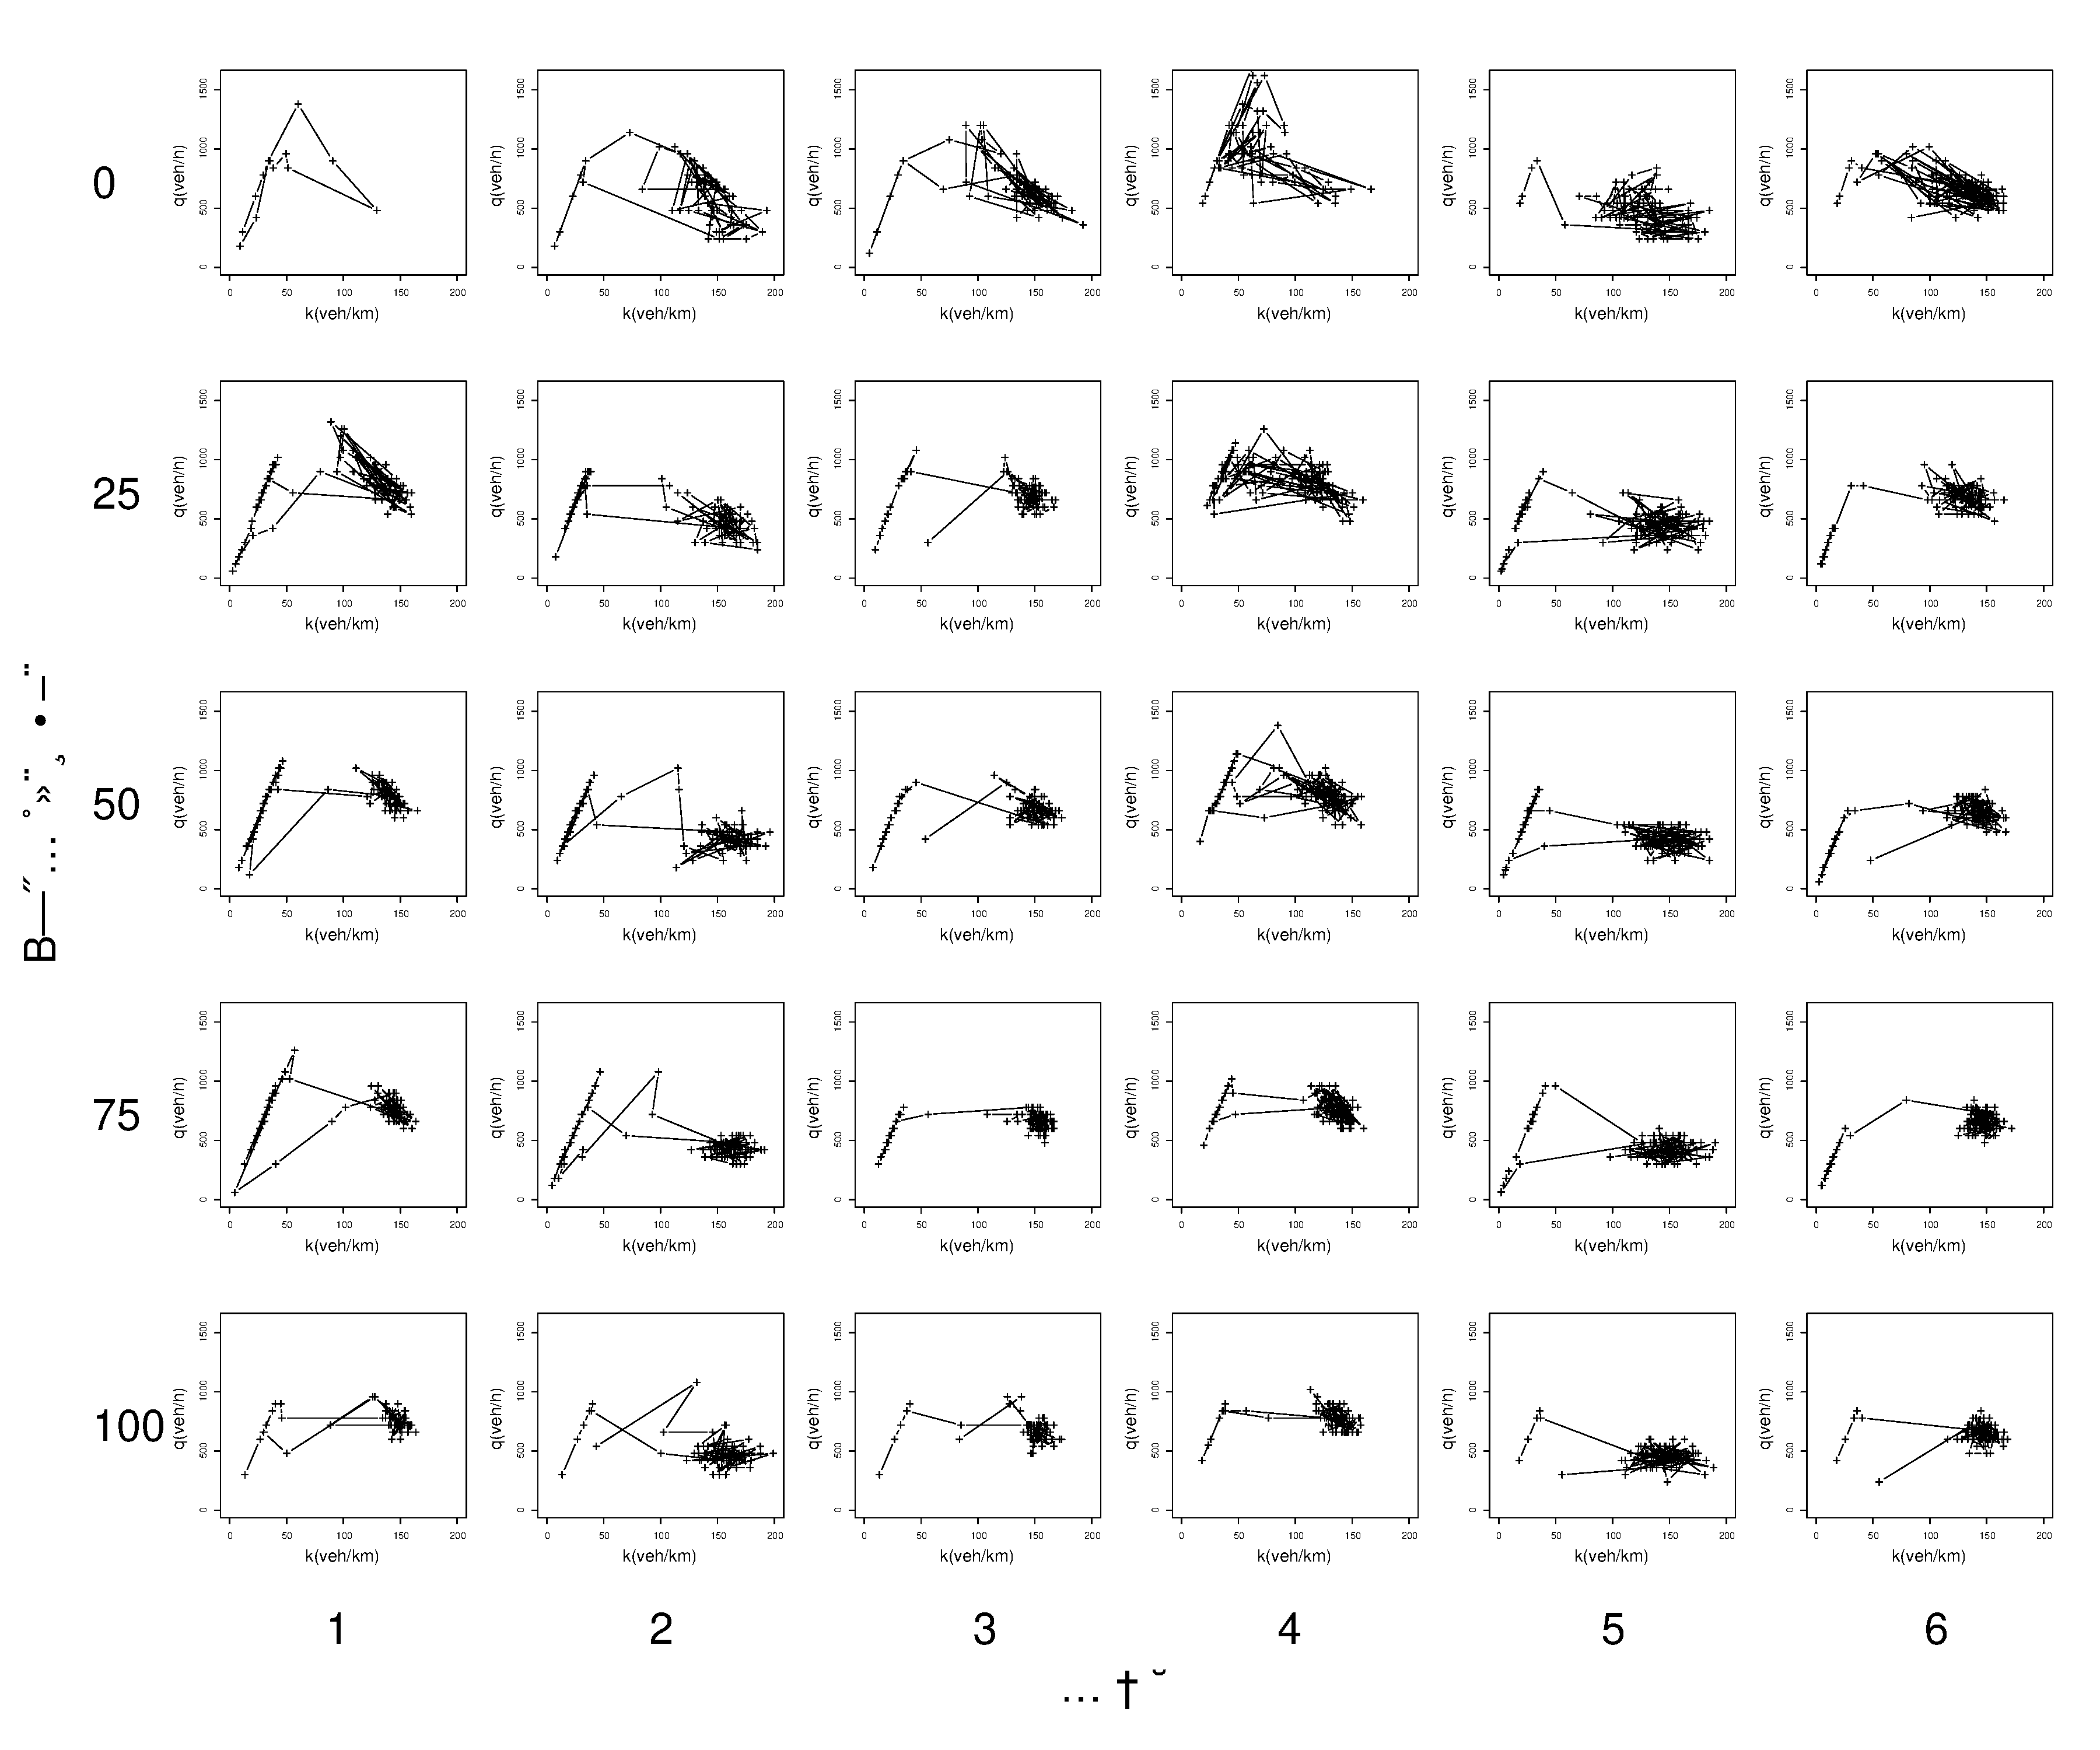
\includegraphics[width=\linewidth]{combined_kqedges}
\caption{混合作用影响下各检测器密度流量关系图}
\label{combined_kqedges}
\end{center}
\end{figure}

\section{对交通流安全性}

评价交通流安全性,使用了TTC倒数的一分钟和值,以及6个检测器流量的一分钟平均值。

TTC倒数的时间平均产生密度,

\subsection{期望速度影响因素}

期望速度从\autoref{factor1_ttc}流量与TTC倒数关系图看,TTC倒数的和值的绝对值最大主要出现在流量600-800之间,从图上看对其分布没有显著影响。由\autoref{factor1_box_avttc}可以看出,期望车速对,时间平均TTC倒数(或者说TTC倒数的时间产生密度)的绝对值有显著的影响,随着期望车速较高的B型驾驶人更多的混入,时间平均TTC倒数的绝对值呈现增加的趋势。当B型驾驶人的比例小于50\%时,使用不同随机数的情况差异较大,说明车辆的顺序对时间平均TTC倒数产生显著的影响。可以理解为低期望车速阻碍高期望车速的作用在B型驾驶人较少时,对交通流的安全性产生较大增加随机性的影响。

\begin{figure}[!htb]%
\centering
\subfloat[][]{
\label{factor1_ttc_per0}%
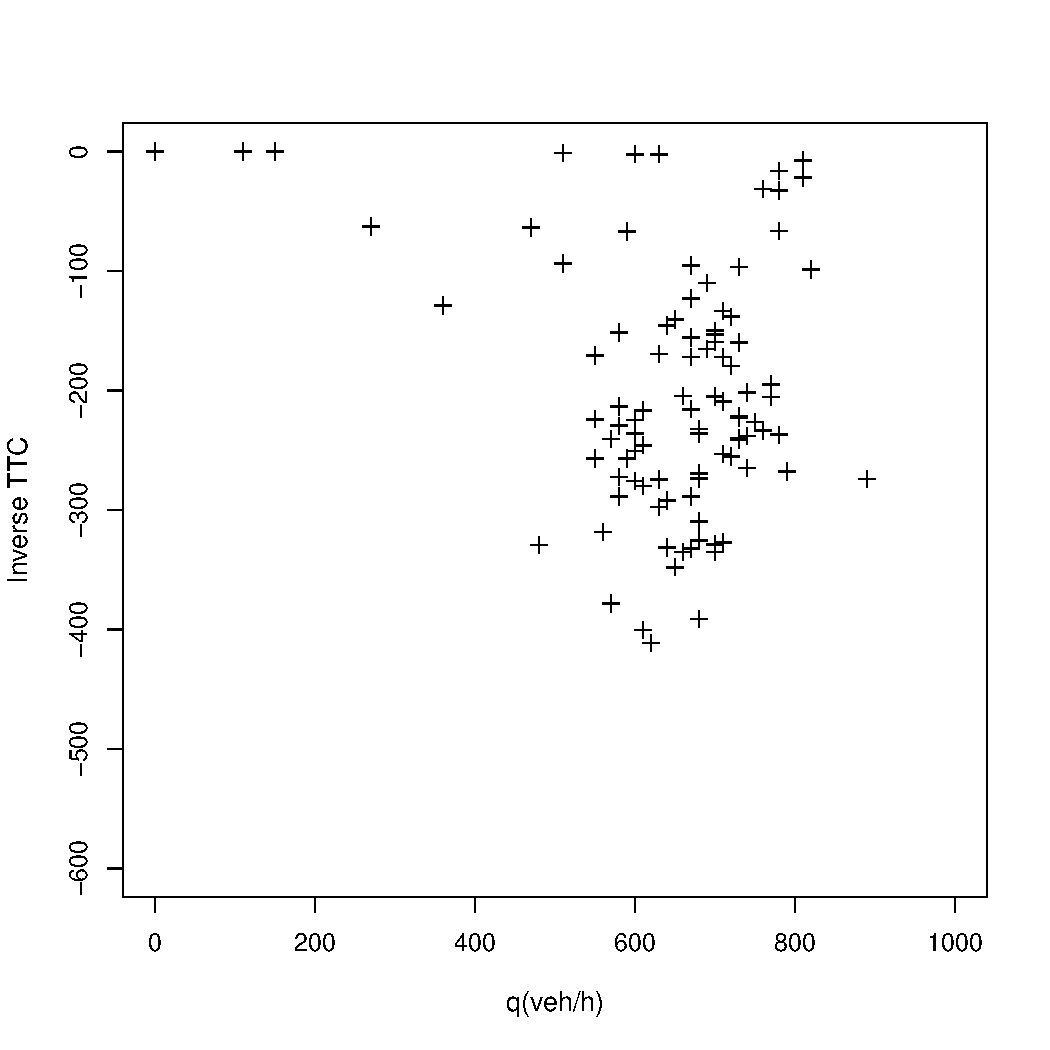
\includegraphics[width=0.33\linewidth]{factor1_ttc_per0}
}%
\subfloat[][]{%
\label{factor1_ttc_per25}%
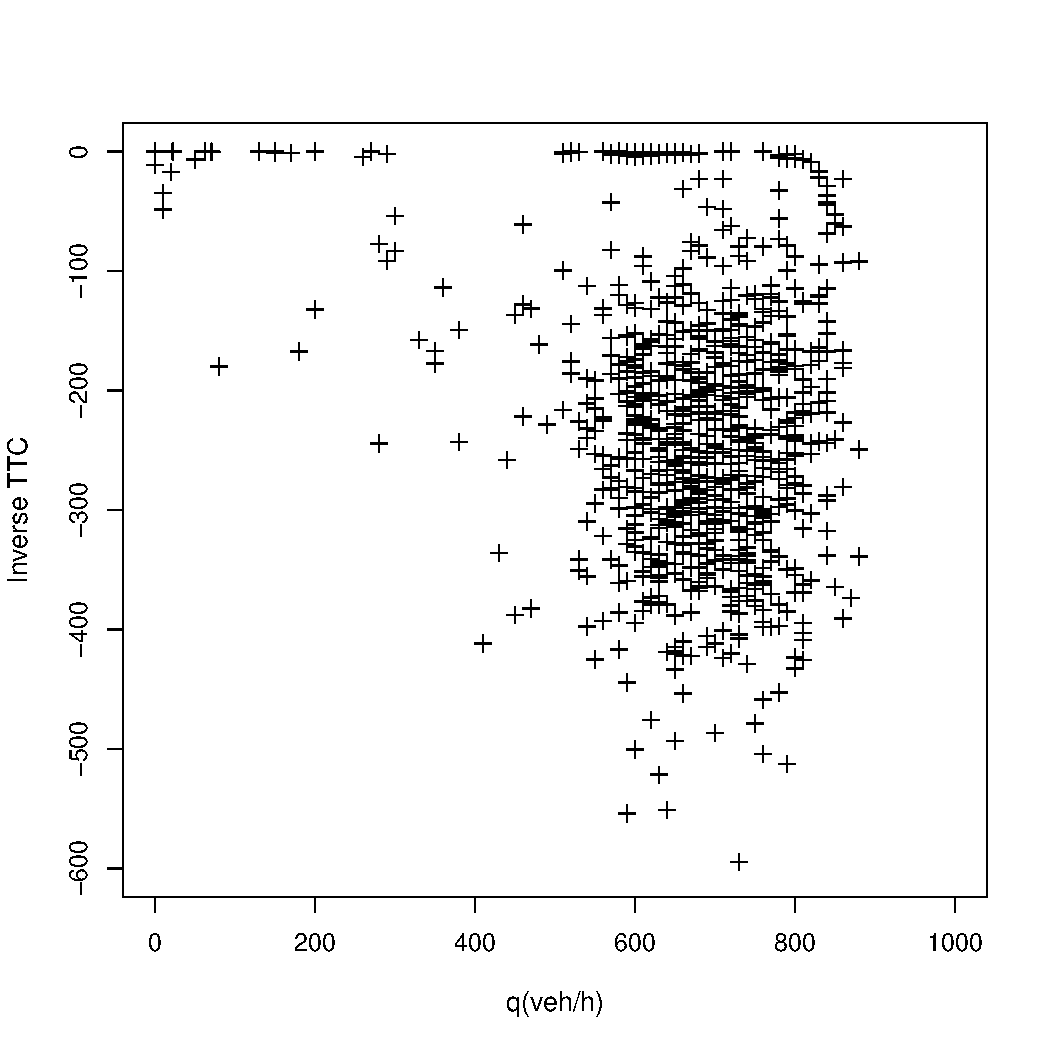
\includegraphics[width=0.33\linewidth]{factor1_ttc_per25}}
\subfloat[][]{%
\label{factor1_ttc_per50}%
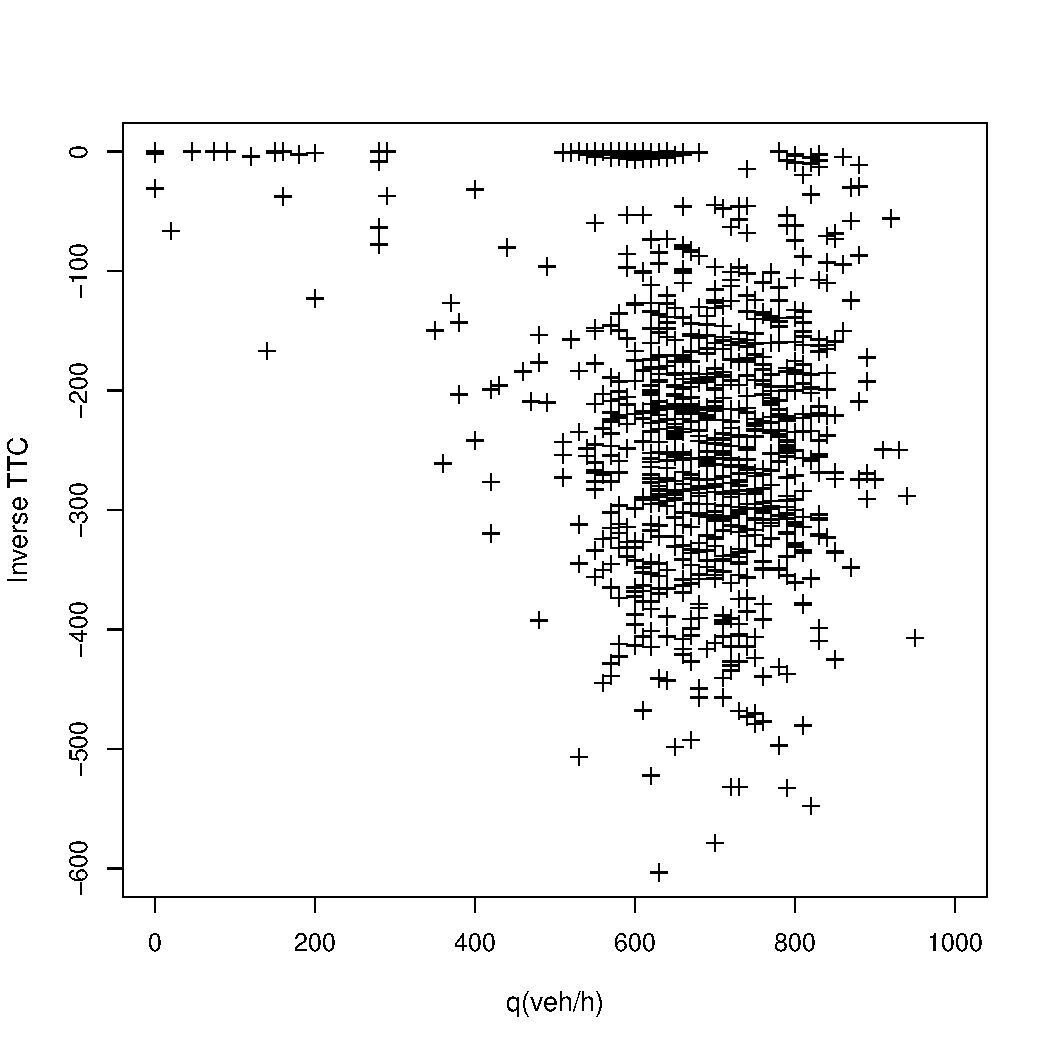
\includegraphics[width=0.33\linewidth]{factor1_ttc_per50}}\\%
\subfloat[][]{%
\label{factor1_ttc_per75}%
\includegraphics[width=0.33\linewidth]{factor1_ttc_per75}}%
\subfloat[][]{%
\label{factor1_ttc_per100}%
\includegraphics[width=0.33\linewidth]{factor1_ttc_per100}}
\caption[A set of four sub-floats.]{期望速度影响下流量与TTC倒数关系图
\subref{factor1_ttc_per0}
\subref{factor1_ttc_per25} 
\subref{factor1_ttc_per50}
\subref{factor1_ttc_per75}
\subref{factor1_ttc_per100}分别表示\autoref{speed-factor}中的B型驾驶人的百分比分别为0\%,25\%,50\%,75\%,100\%,其中流量为6个检测器平均值,TTC倒数为1分钟累计值}%
\label{factor1_ttc}%
\end{figure}

\begin{figure}[!htb]
\begin{center}
\includegraphics[width=0.7\linewidth]{factor1_box_avttc}
\caption{期望速度影响下时间平均TTC倒数箱图}
\label{factor1_box_avttc}
\end{center}
\end{figure}

\subsection{最大减速度影响因素}

最大减速度从\autoref{factor2_ttc}流量与TTC倒数关系图看,TTC倒数的和值的绝对值最大主要出现在流量600左右,从图上看对其分布没有显著影响。由\autoref{factor2_box_avttc}可以看出,期望车速对,时间平均TTC倒数(或者说TTC倒数的时间产生密度)的绝对值呈现先减少后增加的趋势,随着期望车速较高的B型驾驶人更多的混入,时间平均TTC倒数的绝对值呈现先减小后增加的趋势。这似乎说明存在一个最佳的B型驾驶人混入比例使得TTC倒数的实践产生密度绝对值最小。
\begin{figure}[!htb]%
\centering
\subfloat[][]{
\label{factor2_ttc_per0}%
\includegraphics[width=0.33\linewidth]{factor2_ttc_per0}
}%
\subfloat[][]{%
\label{factor2_ttc_per25}%
\includegraphics[width=0.33\linewidth]{factor2_ttc_per25}}
\subfloat[][]{%
\label{factor2_ttc_per50}%
\includegraphics[width=0.33\linewidth]{factor2_ttc_per50}}\\%
\subfloat[][]{%
\label{factor2_ttc_per75}%
\includegraphics[width=0.33\linewidth]{factor2_ttc_per75}}%
\subfloat[][]{%
\label{factor2_ttc_per100}%
\includegraphics[width=0.33\linewidth]{factor2_ttc_per100}}
\caption[A set of four sub-floats.]{最大减速度影响下流量与TTC倒数关系图
\subref{factor2_ttc_per0}
\subref{factor2_ttc_per25} 
\subref{factor2_ttc_per50}
\subref{factor2_ttc_per75}
\subref{factor2_ttc_per100}分别表示\autoref{decel-factor}中的B型驾驶人的百分比分别为0\%,25\%,50\%,75\%,100\%,其中流量为6个检测器平均值,TTC倒数为1分钟累计值}%
\label{factor2_ttc}%
\end{figure}

\begin{figure}[!htb]
\begin{center}
\includegraphics[width=0.7\linewidth]{factor2_box_avttc}
\caption{最大减速度影响下时间平均TTC倒数箱图}
\label{factor2_box_avttc}
\end{center}
\end{figure}

\subsection{混合影响因素}

混合作用影响下的结果与最大减速影响的结果相似,这再一次表明最大减速度是影响交通流的主要因素。
\begin{figure}[!htb]%
\centering
\subfloat[][]{
\label{combined_ttc_per0}%
\includegraphics[width=0.33\linewidth]{combined_ttc_per0}
}%
\subfloat[][]{%
\label{combined_ttc_per25}%
\includegraphics[width=0.33\linewidth]{combined_ttc_per25}}
\subfloat[][]{%
\label{combined_ttc_per50}%
\includegraphics[width=0.33\linewidth]{combined_ttc_per50}}\\%
\subfloat[][]{%
\label{combined_ttc_per75}%
\includegraphics[width=0.33\linewidth]{combined_ttc_per75}}%
\subfloat[][]{%
\label{combined_ttc_per100}%
\includegraphics[width=0.33\linewidth]{combined_ttc_per100}}
\caption[A set of four sub-floats.]{混合作用影响下流量与TTC倒数关系图
\subref{combined_ttc_per0}
\subref{combined_ttc_per25} 
\subref{combined_ttc_per50}
\subref{combined_ttc_per75}
\subref{combined_ttc_per100}分别表示\autoref{combined-factor}中的B型驾驶人的百分比分别为0\%,25\%,50\%,75\%,100\%,其中流量为6个检测器平均值,TTC倒数为1分钟累计值}%
\label{combined_ttc}%
\end{figure}

\begin{figure}[!htb]
\begin{center}
\includegraphics[width=0.7\linewidth]{combined_box_avttc}
\caption{混合作用影响下时间平均TTC倒数箱图}
\label{combined_box_avttc}
\end{center}
\end{figure}

\section{本章小结}



%\begin{figure}[htb] 
%  \begin{minipage}[b]{0.3\linewidth} 
%
%  \end{minipage}% 
%  \begin{minipage}[b]{0.3\linewidth} 
%
%  \end{minipage} 
%  \begin{minipage}[b]{0.3\linewidth} 
%
%  \end{minipage} 
%\end{figure}



%\begin{figure}[htb] 
%  \begin{minipage}[b]{0.33\linewidth} 
%\begin{center}
%\includegraphics[width=\linewidth]{factor1_vq_per0}
%\end{center}
%\caption{模拟场景图}
%\label{factor1_vq_per0}
%  \end{minipage}% 
%  \begin{minipage}[b]{0.33\linewidth} 
%\begin{center}
%\includegraphics[width=\linewidth]{factor1_vq_per25}
%\end{center}
%\caption{模拟场景图}
%\label{factor1_vq_per25}
%  \end{minipage} 
%  \begin{minipage}[b]{0.33\linewidth} 
%\begin{center}
%\includegraphics[width=\linewidth]{factor1_vq_per50}
%\end{center}
%\caption{模拟场景图}
%\label{factor1_vq_per50}
%  \end{minipage}
%\hspace*{0.17\linewidth}
%  \begin{minipage}[b]{0.33\linewidth} 
%\begin{center}
%\includegraphics[width=\linewidth]{factor1_vq_per75}
%\end{center}
%\caption{模拟场景图}
%\label{factor1_vq_per75}
%  \end{minipage}
%  \begin{minipage}[b]{0.33\linewidth} 
%\begin{center}
%\includegraphics[width=\linewidth]{factor1_vq_per100}
%\end{center}
%\caption{模拟场景图}
%\label{factor1_vq_per100}
%  \end{minipage}
%\end{figure}
\chapter{结论与展望}
\section{主要成果}

\section{研究所存在的问题}


\section{研究展望}

\end{Main} % 结束正文

\begin{Thanks}
历经一年的时间,论文已接近尾声,同时两年半的硕士研究生生活在这个季节也即将划上句号,而于我的人生却只是一个逗号,我将面对又一次征程的开始。在此,我要向我的家人、老师、同学、朋友表达我最诚挚的感谢!是你们让我感到了温暖,是你们让我有了前进的力量,是你们让我的读研生活如此精彩。
首先我要感谢我的指导老师陆建教授。在两年半的研究生生活中,陆老师无论在学术上,还是在生活中,都对我关怀备至,使我得到很大的提高。陆老师治学严谨,知识渊博,恭谦近人,是我的良师益友,更是我学习的楷模。在陆老师身上学习到的不仅是专业的知识,更多的是做人做事的道理,对我今后的人生道路将产生长远的影响。论文的完成得到陆老师无微不至的关心与指导,从论文的开题、实验的设计、仪器的准备到具体的研究工作,无不倾注了陆老师大量的心血!在论文完成之际,谨向尊敬的陆老师致以我最诚挚的谢意与衷心的祝福!
论文的完成还得到了姜军师兄和吴璠同学的大力支持,姜军师兄如兄长般的关怀,在关键时刻对我的指点,吴璠同学对我不遗余力的帮助,使得我能够顺利的完成论文。借此机会,在此表示我深深的谢意。
感谢王炜院长、过秀成老师、陈学武老师、任刚老师、陈峻老师、邓卫老师、李文权老师、陈琳老师、项乔君老师、胡晓健老师、王昊老师、杨敏老师,在东南大学的求学岁月里,教给了我学术上的相关专业知识以及探求知识的方法。
感谢秦霞书记、张建老师、陈怡老师、沈溶老师、黄宏老师、罗磊老师,为交通学院营造出一个大家庭的氛围,以及对我的关怀,让我在近七年的大学生活中,感受到切实的家一般的温暖。
感谢课题组的孙祥龙师兄、杨海飞师兄、赵勇同学、周成彦同学、李文华同学、杜璇同学对我的支持与照顾,感谢宿舍兄弟侯现耀、张磊、方程炜对我的帮助与关怀,能与你们共度这最美好的读研时光,是我的幸运与幸福。
最后特别要感谢我的父亲、母亲和姐姐,是你们一直以来默默无闻的付出和一贯的支持与鼓励,才使我能够一步一步的成长,才使我有信心和毅力完成学业,无论今后我身在何方,心中不变的思念,永远是相同的地方。
谨以此文献给所有关心、支持我的人,我将更加努力,不辜负大家的期望。
胡武林 

\end{Thanks}

\bibliography{seuthesis}
%\bibliographystyle{seuthesis}

\begin{Appendix}
  \chapter{受调查驾驶人基本情况}% latex table generated in R 2.12.0 by xtable 1.5-6 package
% Thu Mar 03 12:36:06 2011
\begin{table}[ht]
\begin{center}
\begin{tabular}{ccccccc}
  \hline
编号 & 性别 & 年龄 & 驾照类型 & 驾龄(年) & 累计行驶里程(万公里) & 是否专业驾驶人 \\ 
  \hline
  1 & 女 & 25 & C1 & 0 & 0.0 & 否 \\ 
  2 & 男 & 23 & C1 & 1 & 0.5 & 否 \\ 
  3 & 男 & 26 & C1 & 4 & 2.0 & 否 \\ 
  4 & 女 & 24 & C1 & 2 & NA & 否 \\ 
  5 & 男 & 24 & C1 & 4 & 0.6 & 否 \\ 
  6 & 男 & 26 & C1 & 5 & 1.0 & 否 \\ 
  7 & 男 & 26 & C1 & 4 & 0.5 & 否 \\ 
  8 & 男 & 23 & C1 & 4 & 0.2 & 否 \\ 
  9 & 男 & 24 & C1 & 5 & 1.5 & 否 \\ 
 10 & 男 & 24 & C1 & 3 & 1.0 & 否 \\ 
 11 & 男 & 28 & C1 & 1 & 0.5 & 否 \\ 
 12 & 男 & 25 & C1 & 1 & 0.8 & 否 \\ 
 13 & 女 & 24 & C1 & 3 & 2.5 & 否 \\ 
 14 & 男 & 24 & C1 & 2 & 2.0 & 否 \\ 
 15 & 男 & 29 & C1 & 5 & NA & 否 \\ 
 16 & 男 & 25 & C1 & 4 & 15.0 & 否 \\ 
 17 & 男 & 39 & NA & 3 & 24.0 & 是 \\ 
 18 & 男 & 44 & A & 11 & 90.0 & 是 \\ 
 19 & 男 & 37 & A & 10 & NA & 是 \\ 
 20 & 男 & 33 & B & 16 & 30.0 & 是 \\ 
 21 & 男 & 43 & B & 6& 60.0 & 是 \\ 
 22 & 男 & 45 & A & 23 & 200.0 & 是 \\ 
 23 & 男 & NA & A & 10 & 50.0 & 是 \\ 
 24 & 男 & 50 & NA & 14 & 15.0 & 是 \\ 
 25 & 男 & 53 & NA & 18 & 60.0 & 是 \\ 
 26 & 男 & 47 & A & 15 & 76.0 & 是 \\ 
   \hline
\end{tabular}
\label{basic_table}
\end{center}
\end{table}

%  \chapter{第二个附录}
%  ……
\end{Appendix}

\newpage
\printindex % 索引

\begin{Resume}
作者简介
\end{Resume}
\backcover
\end{document}
